\chapter{Method Validation} \label{chap:validation} \minitoc

In this section, we provide summary statistics for our method's performance and draw visualizations for the obtained results to validate our alarms and reason about them.

\section{Experiments with Synthetic Data}
In order to test our proposed system, we generated multiple synthetic datasets before moving on to real data. In this section, we present summary statistics for the synthetic datasets created and our generated alarms.

\subsection{Single-Feature Analysis}
As an initial step, we started by validating our system using single-feature datasets before moving to multi-feature scenarios to facilitate system validation, considering the complexities of multi-feature datasets and the problem of multiple test correction. In this section, we validate our results for single-feature synthetic datasets.

\subsubsection{Varying Sample Sizes}
We began with single-feature scenarios and by experimenting with different tuple-based half-lives $n_{1/2}$. The half-life $n_{1/2}$ parameter in turn controls the size of the samples we make in the batch phase and the target sliding window size of the streaming phase. 

In Section \ref{sec:ema-hist}, we mentioned that we choose to discard events whose contribution is less than 6\%. We set a half-life $n_{1/2}$ value and then multiply it by a constant factor of 4 to get the size of the samples to make (a larger sample would contain events whose contribution was equal to or less than 6\%). 

All the synthetic datasets used throughout this section are a time-series where at each time-step we sample uniformly from a fixed distribution, \textit{i.e.}, there are no time correlations in the used datasets. The reference dataset R1 used in this first experiment contained a single feature that followed a normal distribution with mean $\mu=10$ and standard deviation $\sigma=2$ for the 5 million rows of the dataset. Figure \ref{fig:timeseries-r1} shows the time-series of the single feature in dataset R1. The dataset processed in the streaming phase (\textit{i.e.}, the target dataset) was generated with a size of 5 million events and a single feature. For the first half, \textit{i.e.}, for the first 2.5 million events, the feature followed a normal distribution with mean $\mu=10$ and standard deviation $\sigma=2$, like the reference dataset. For the other half, we changed the generating distribution to be a continuous uniform one with lower bound $a=100$ and upper bound $b=200$. Figure \ref{fig:timeseries-t1} shows the time-series of the single feature in the target dataset T1 where we see the abrupt change in feature values.
\begin{center}
\begin{minipage}{.5\textwidth}
  \centering
  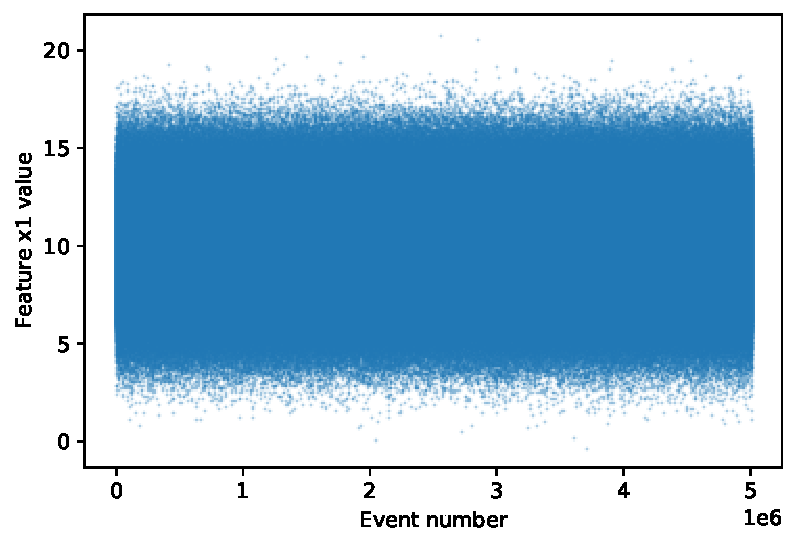
\includegraphics[width=1\linewidth]{figures/01-reference.pdf}
  \captionof{figure}{Time-series for dataset R1}
  \label{fig:timeseries-r1}
\end{minipage}%
\begin{minipage}{.5\textwidth}
  \centering
  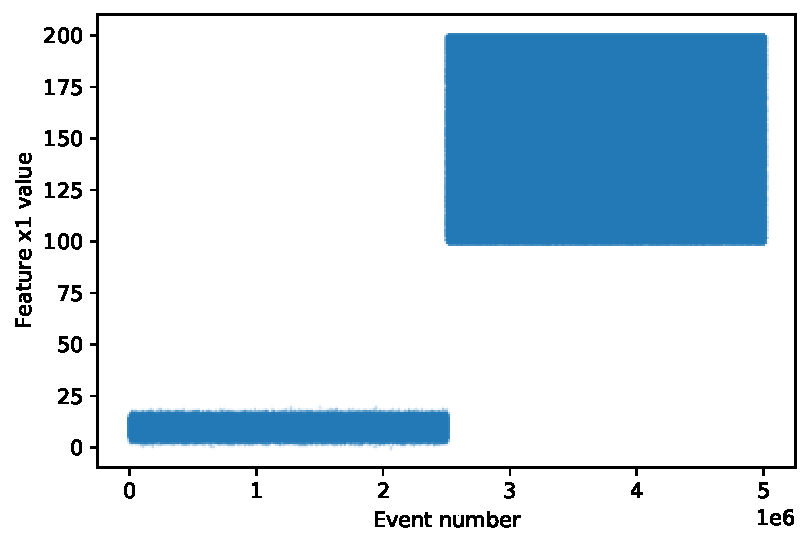
\includegraphics[width=1\linewidth]{figures/01-target.pdf}
  \captionof{figure}{Time-series for dataset T1}
  \label{fig:timeseries-t1}
\end{minipage}
\end{center}

We conducted three different experiments varying the tuple-based half-life $n_{1/2}$, using the reference dataset R1 and the target dataset T1. The experiment identifiers, the corresponding half-lives and the execution times are shown in Table \ref{tbl:tests-half-life}. Notice that $Sample Size$ corresponds to the size of each sample made in the batch phase and so it is four times the half-life. We used 100 bins (plus the two special infinity bins) for the reference histogram and made 1000 samples.
\begin{table}[!htb]
    \begin{center}
        \begin{tabular}{|c|c|c|c|c|}
        \hline
        \multicolumn{1}{|l|}{\textbf{Experiment}} & \multicolumn{1}{l|}{\textbf{Half-life}} & \multicolumn{1}{l|}{\textbf{Sample Size}} & \multicolumn{1}{l|}{\textbf{Executors}} & \multicolumn{1}{l|}{\textbf{Batch execution time (seconds)}} \\ \hline
        01                                        & 625                                     & 2500                                      & 300                                     & 152                                                          \\ \hline
        02                                        & 62,500                                  & 250,000                                   & 300                                     & 2,822                                                        \\ \hline
        03                                        & 250,000                                 & 1,000,000                                 & 300                                     & 10,082                                                       \\ \hline
        \end{tabular}
    \end{center}
    \caption{Experiments with varying half-life}
    \label{tbl:tests-half-life}
\end{table}
Table \ref{tbl:tests-half-life} shows the execution time for the batch phase in seconds. All experiments used 300 Spark executor instances. From the Table we conclude that the larger the half-life, the larger the sample size. Larger samples imply longer processing times when computing the EMA-like histogram for each sample. With no surprise, we see that the larger the sample the longer it takes to finish the batch phase.

From a functional point of view, were we able to detect the abrupt change introduced in the target dataset T1? Recall that from the 2.5 millionth event forward we change the distribution from a gaussian to an uniform one (Figure \ref{fig:timeseries-t1}). Figure \ref{fig:JSD-signal-01} shows the distance (JSD) values computed during streaming at each event of the 5 million events from dataset T1, using the outputs from the batch phase of experiment 01. We clearly see a change in JSD values, and we move from values close to 0 to values close to 1 (or even 1). Figure \ref{fig:JSD-signal-zoom-01} shows the same signal but for the first half of the streaming period (essentially a zoom-in). We see our JSD values before the change were very low (magnitudes of $10^{-2}$).
\begin{figure}[!htb]
\centering
\begin{subfigure}{.5\textwidth}
  \centering
  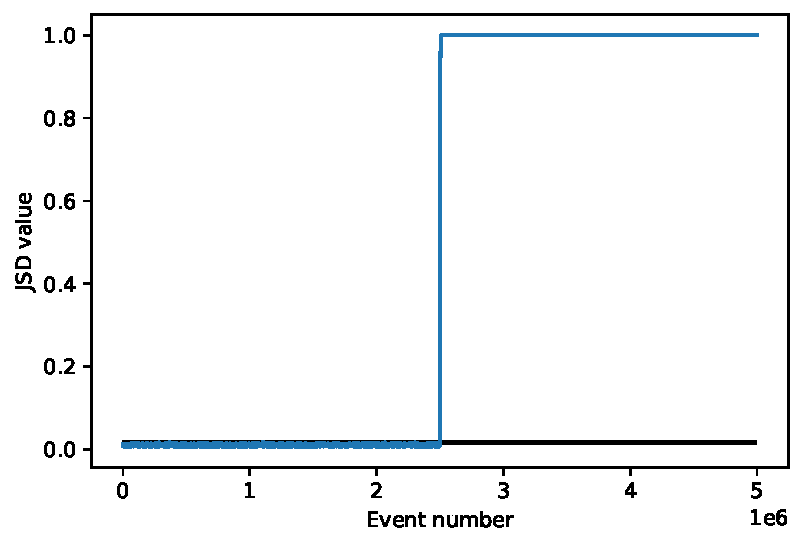
\includegraphics[width=1\linewidth]{figures/stream-analysis-viz-625.pdf}
  \caption{For the whole time-series}
  \label{fig:JSD-signal-01}
\end{subfigure}%
\begin{subfigure}{.5\textwidth}
  \centering
  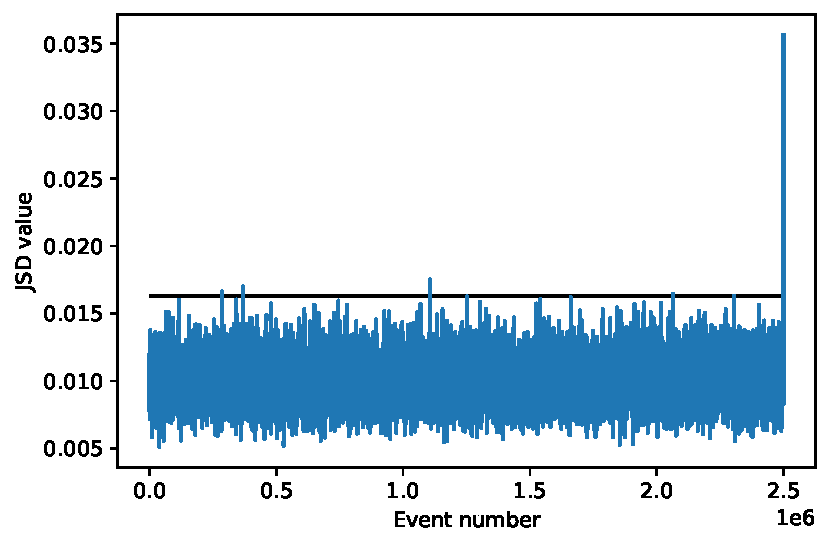
\includegraphics[width=1\linewidth]{figures/stream-analysis-viz-zoom-625.pdf}
  \caption{Zoom in on the first 2.5 million events}
  \label{fig:JSD-signal-zoom-01}
\end{subfigure}
\caption{Experiment 01: JSD signal and threshold}
\end{figure}

However, the change in JSD value is very abrupt as well. Almost instantly we go from close to 0 values to 1. We also had some false-positives, \textit{i.e.}, some JSD values above the threshold. This indicates to us that the window used is too small and sensitive to small changes, or that we can choose a more strict threshold.

In experiment 02, we use larger sampling windows. Remember our target sliding window in streaming is of the same size as the sampling windows. In the second experiment, we increase the size of the sampling and target windows by 100 times.

Figure \ref{fig:JSD-signal-02} shows the JSD signal during streaming for dataset T1, using the outputs from the batch phase of experiment 02. Again, we see a change in signal from the middle of the streaming period forward. Figure \ref{fig:JSD-signal-zoom-02} shows the same signal for the first half of the streaming period.
\begin{figure}[!htb]
\centering
\begin{subfigure}{.5\textwidth}
  \centering
  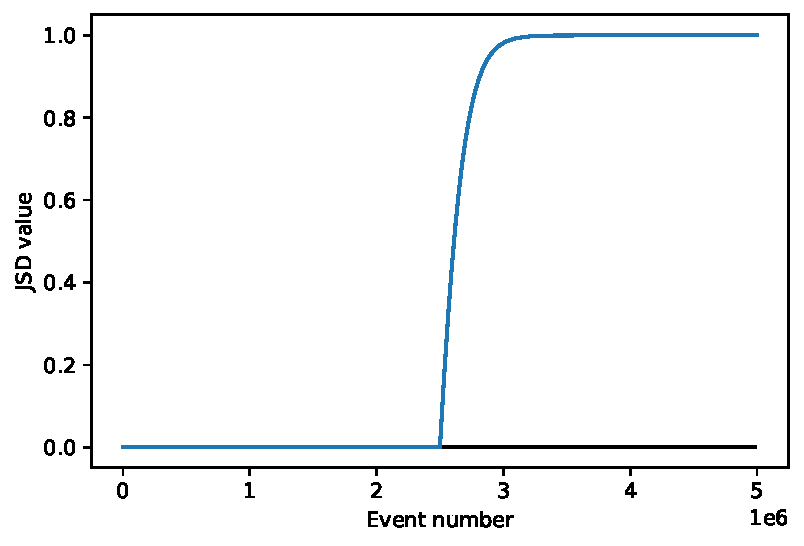
\includegraphics[width=1\linewidth]{figures/stream-analysis-viz-62500.pdf}
  \caption{For the whole time-series}
  \label{fig:JSD-signal-02}
\end{subfigure}%
\begin{subfigure}{.5\textwidth}
  \centering
  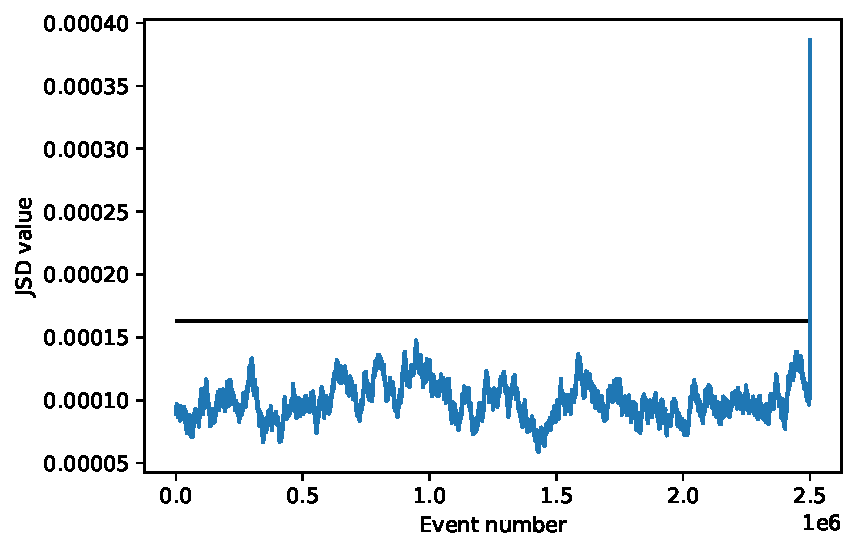
\includegraphics[width=1\linewidth]{figures/stream-analysis-viz-zoom-62500.pdf}
  \caption{Zoom in on the first 2.5 million events}
  \label{fig:JSD-signal-zoom-02}
\end{subfigure}
\caption{Experiment 02: JSD signal and threshold}
\end{figure}
Notice that this time the growth of our signal is slower. Notice also that we do not have false positives in the first half of the signal. This is because we use a larger window, which means each event has a smaller contribution to the aggregation state. Hence, outliers will have less impact on the aggregation and corresponding signal value.

In experiment 03, we increase the sampling and target windows size once again, this time four times larger than in experiment 02. We would expect an even smoother growth of our signal and, again, no false positives. And indeed, judging by the corresponding signal computation and zoom-in, Figures \ref{fig:JSD-signal-03} and \ref{fig:JSD-signal-zoom-03}, respectively, the signal looks smoother and we see no false positives.
\begin{figure}[!htb]
\centering
\begin{subfigure}{.5\textwidth}
  \centering
  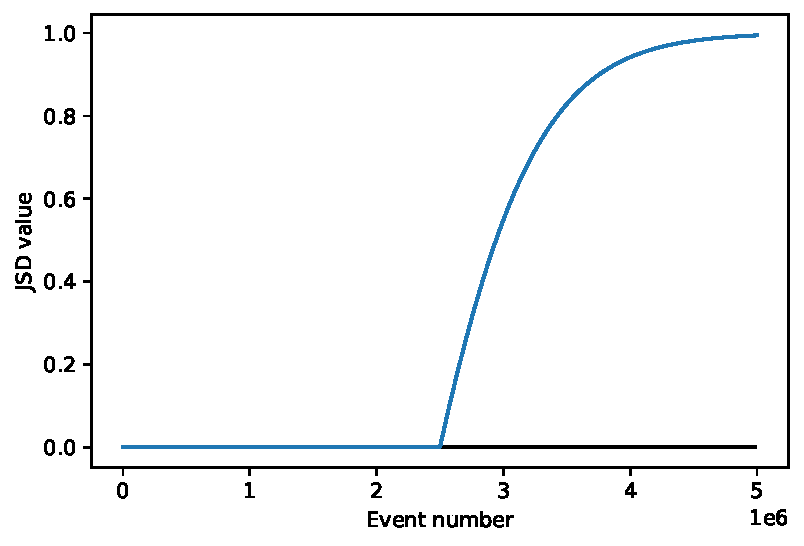
\includegraphics[width=1\linewidth]{figures/stream-analysis-viz-250000.pdf}
  \caption{For the whole time-series}
  \label{fig:JSD-signal-03}
\end{subfigure}%
\begin{subfigure}{.5\textwidth}
  \centering
  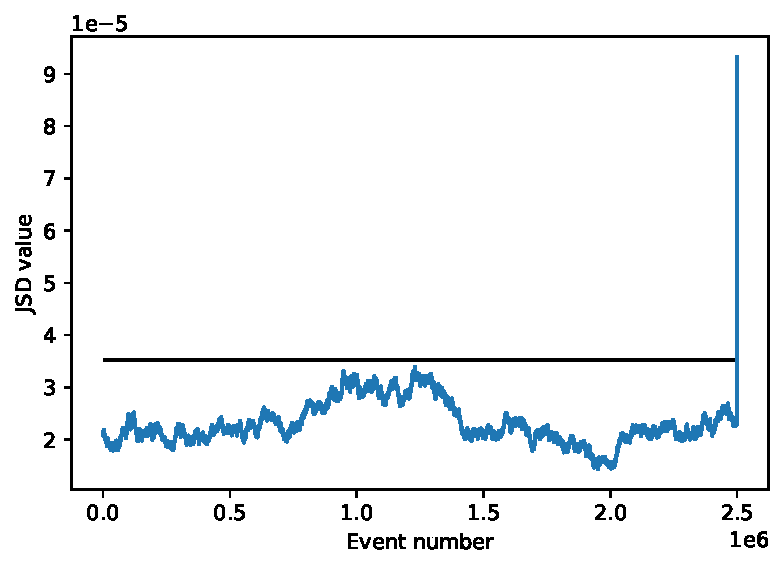
\includegraphics[width=1\linewidth]{figures/stream-analysis-viz-zoom-250000.pdf}
  \caption{Zoom in on the first 2.5 million events}
  \label{fig:JSD-signal-zoom-03}
\end{subfigure}
\caption{Experiment 03: JSD signal and threshold}
\end{figure}


\subsubsection{Multiple Distribution Changes}
In this experiment, we wanted to see how our signal behaved when there were multiple change points, where each gaussian distribution was a scaled down version of the previous one. Figure \ref{fig:timeseries-r2} shows the time-series for the reference dataset R2 used in this experiment. It contained 5 million events with a single feature following a gaussian distribution with mean $\mu=100$ and standard deviation $\sigma=50$. The time-series for target dataset T2 is shown in Figure \ref{fig:timeseries-t2}. Notice that we change distributions at 2, 3 and 4 millionth events. Notice also that each subsequent distribution produces values whose domain is a subset of the previous distribution.
\begin{center}
\begin{minipage}{.5\textwidth}
  \centering
  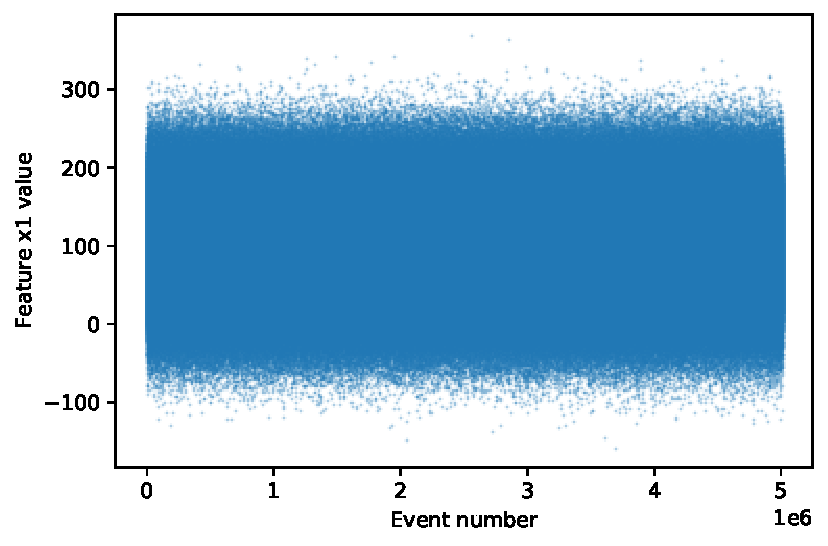
\includegraphics[width=1\linewidth]{figures/timeseries-r2.pdf}
  \captionof{figure}{Time-series for dataset R2}
  \label{fig:timeseries-r2}
\end{minipage}%
\begin{minipage}{.5\textwidth}
  \centering
  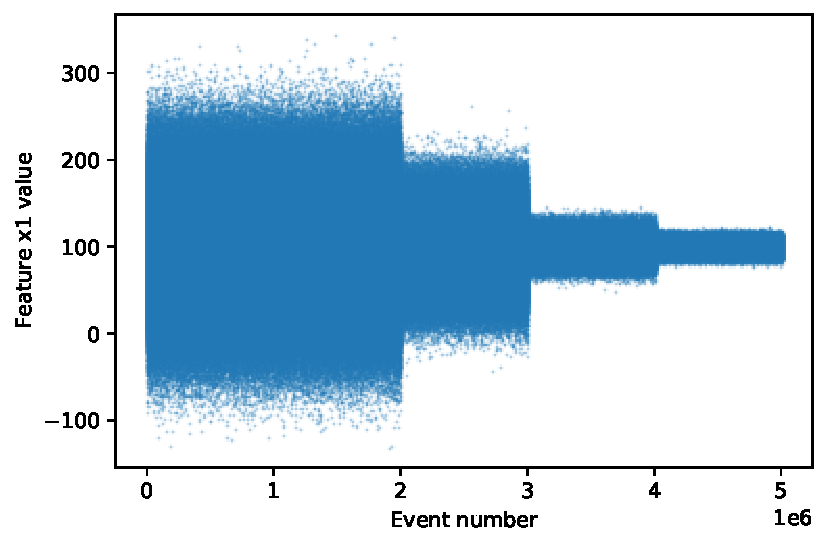
\includegraphics[width=1\linewidth]{figures/timeseries-t2.pdf}
  \captionof{figure}{Time-series for dataset T2}
  \label{fig:timeseries-t2}
\end{minipage}
\end{center}

The target dataset T2 begins with the same distribution as the reference dataset R2, a gaussian distribution with mean $\mu=100$ and standard deviation $\sigma=50$. At the 2 millionth event mark, we use another Gaussian distribution, this time with mean $\mu=100$ and standard deviation $\sigma=30$. At the 3 millionth event, we change the standard deviation to be $\sigma=10$. From the 4 millionth event to the end, we use a standard deviation of $\sigma=5$. 

In this experiment, we used a half-life $n_{1/2}=62500$ and corresponding sample size of 250,000 events, like in the previous section's experiment 02. Figure \ref{fig:JSD-signal-test02} shows the computed JSD signal for the target dataset and Figure \ref{fig:JSD-signal-zoom-test02} zooms in on the first 2 millionth events, before any distribution is changed. We observe that once again we have no false positives in the first 2 million events, which is ideal. 
\begin{figure}[!htb]
\centering
\begin{subfigure}{.5\textwidth}
  \centering
  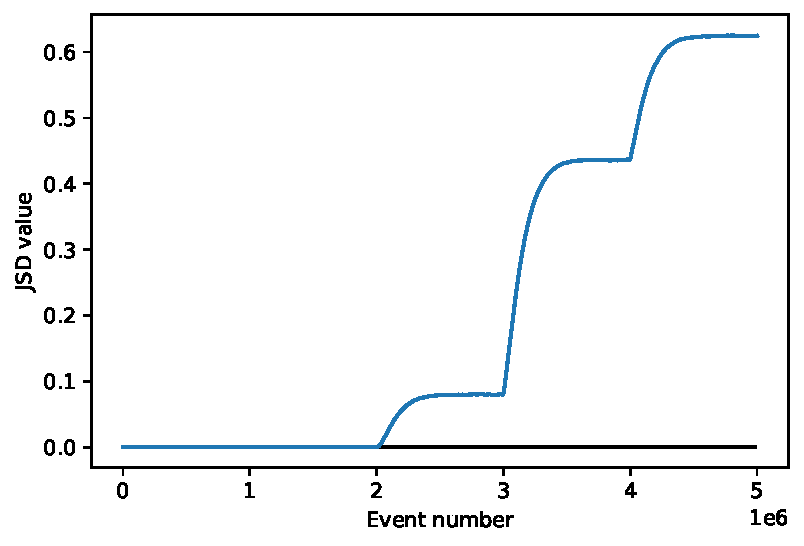
\includegraphics[width=1\linewidth]{figures/stream-analysis-viz-test02.pdf}
  \caption{For the whole time-series}
  \label{fig:JSD-signal-test02}
\end{subfigure}%
\begin{subfigure}{.5\textwidth}
  \centering
  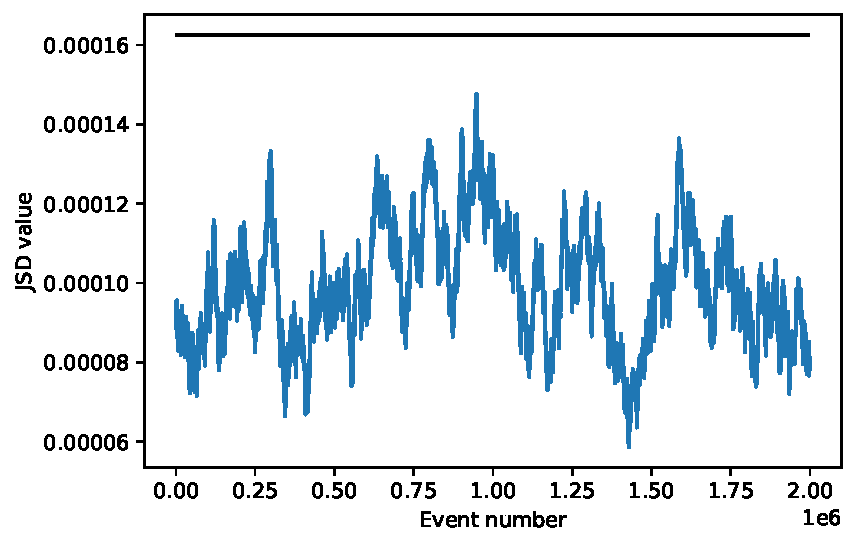
\includegraphics[width=1\linewidth]{figures/stream-analysis-viz-zoom-test02.pdf}
  \caption{Zoom in on the first 2 million events}
  \label{fig:JSD-signal-zoom-test02}
\end{subfigure}
\caption{JSD signal and threshold}
\end{figure}
Furthermore, we observe that the computed JSD signal varies accordingly with the changes in distribution. Despite us changing the distributions to subsets of the previous ones to try and deceive our method, our signal accurately represents these changes. In Figure \ref{fig:JSD-signal-test02}, we see several growth points that correspond to the points where the generating gaussian distribution parameters changed. Hence, we are able to detect changes in distribution parameter changes and quantify how big the change is (the closer to 1 our signal is).

\subsubsection{Multiple Distribution Changes, each a Superset of the Previous One}
In this experiment, we wanted to do the reverse of the previous one. In this one, there are multiple change points but each new distribution spans a domain that is a superset of the previous one. Figure \ref{fig:timeseries-r3} shows the reference period used, with 5 million events and one feature following a gaussian distribution of mean $\mu=100$ and standard deviation $\sigma=10$. Figure \ref{fig:timeseries-t3} shows the target period used, also with 5 million events and one feature. Like in the previous experiment, we change distributions at the 2, 3 and 4 millionth event mark. On the other hand, unlike the previous experiment, we now make subsequent distributions cover the previous ones. We change the reference gaussian used with mean $\mu=100$ and standard deviation $\sigma=10$ at the 2, 3 and 4 millionth mark, to use standard deviations $\sigma=30$, $\sigma=40$ and $\sigma=50$, respectively.
\begin{center}
\begin{minipage}{.5\textwidth}
  \centering
  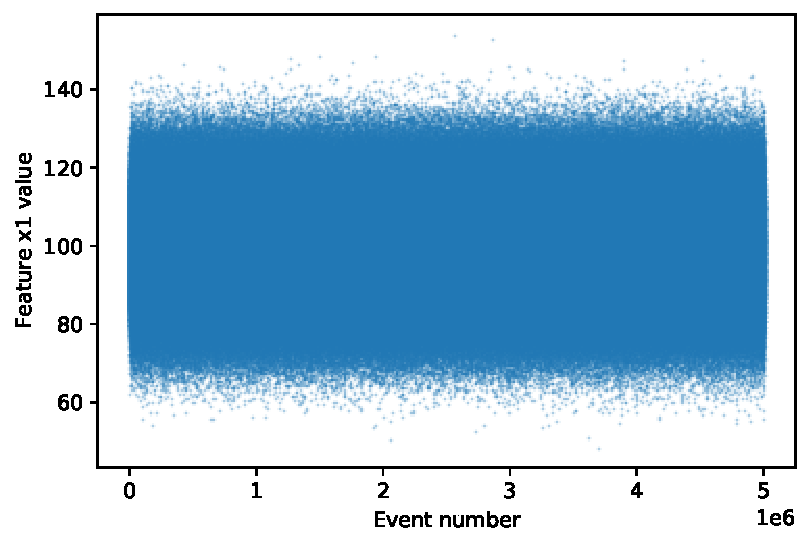
\includegraphics[width=1\linewidth]{figures/timeseries-r3.pdf}
  \captionof{figure}{Time-series for dataset R3}
  \label{fig:timeseries-r3}
\end{minipage}%
\begin{minipage}{.5\textwidth}
  \centering
  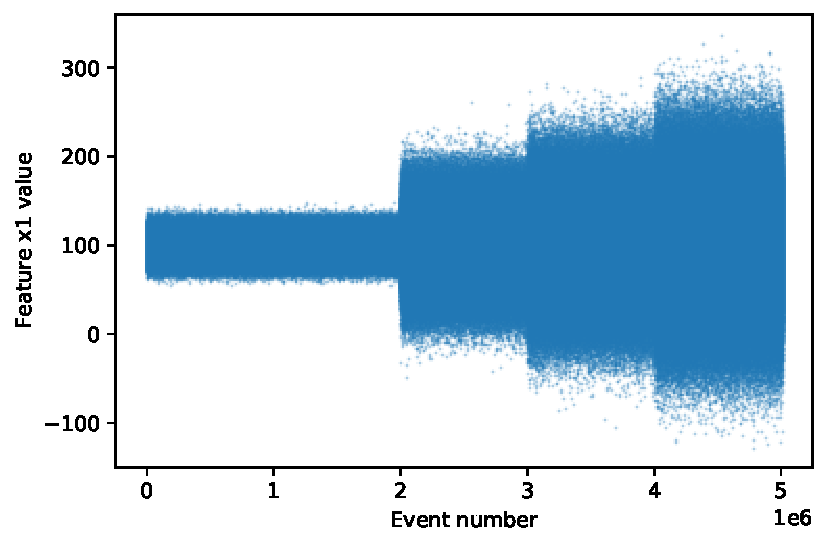
\includegraphics[width=1\linewidth]{figures/timeseries-t3.pdf}
  \captionof{figure}{Time-series for dataset T3}
  \label{fig:timeseries-t3}
\end{minipage}
\end{center}

Figure \ref{fig:JSD-signal-test03} shows the JSD signal for the target dataset in this experiment. Once again, we were able to detect the changes introduced at the 2, 3 and 4 millionth events. We are also able to identify bigger distribution changes, relative to the reference, by observing bigger JSD values. Figure \ref{fig:JSD-signal-zoom-test03} shows a zoomed in portion of the original signal, where we can verify that there are no false positives.
\begin{figure}[!htb]
\centering
\begin{subfigure}{.5\textwidth}
  \centering
  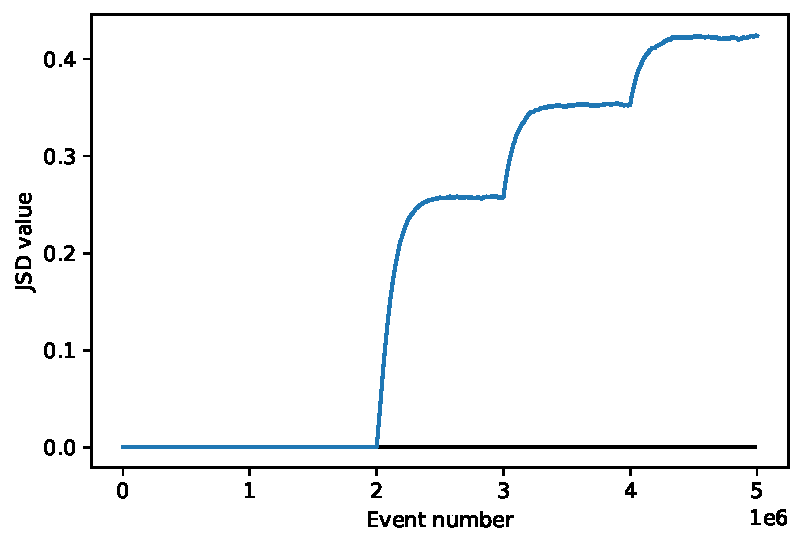
\includegraphics[width=1\linewidth]{figures/stream-analysis-viz-test03.pdf}
  \caption{For the whole time-series}
  \label{fig:JSD-signal-test03}
\end{subfigure}%
\begin{subfigure}{.5\textwidth}
  \centering
  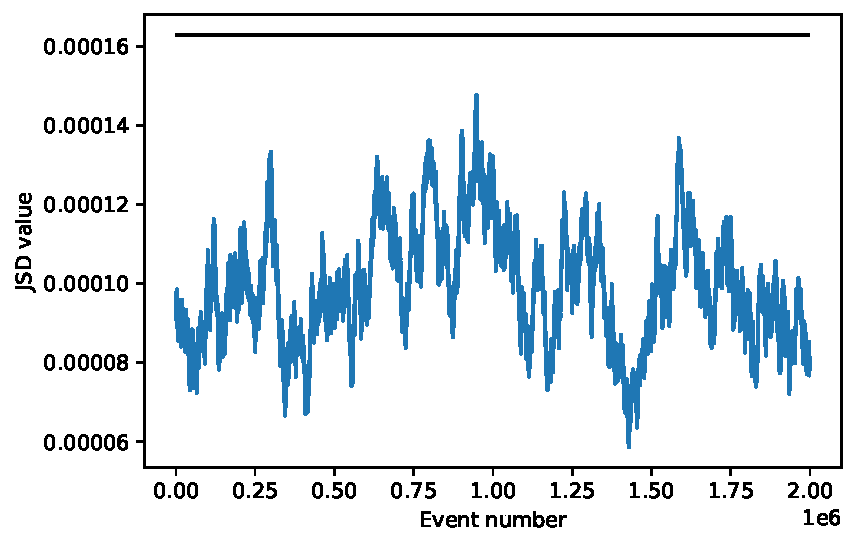
\includegraphics[width=1\linewidth]{figures/stream-analysis-viz-zoom-test03.pdf}
  \caption{Zoom in on the first 2 million events}
  \label{fig:JSD-signal-zoom-test03}
\end{subfigure}
\caption{JSD signal and threshold}
\end{figure}

\subsubsection{Return to Normality After Change}
Our goal with this experiment was to check if our signal returned to its normal values (below the alert threshold) if we changed our distribution to the original reference one, as intended.

In this experiment, we used reference dataset R4 (Figure \ref{fig:timeseries-r4}) and target dataset T4 (Figure \ref{fig:timeseries-t4}). 
\begin{center}
\begin{minipage}{.5\textwidth}
  \centering
  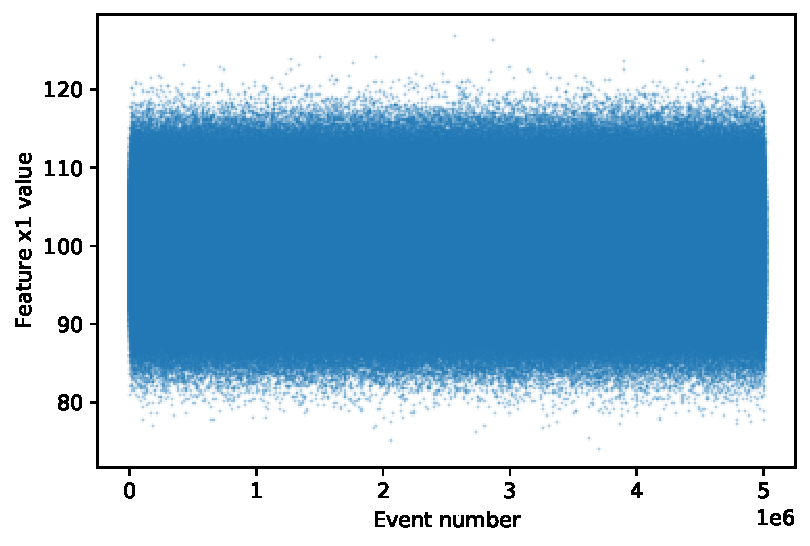
\includegraphics[width=1\linewidth]{figures/timeseries-r4.pdf}
  \captionof{figure}{Time-series for dataset R4}
  \label{fig:timeseries-r4}
\end{minipage}%
\begin{minipage}{.5\textwidth}
  \centering
  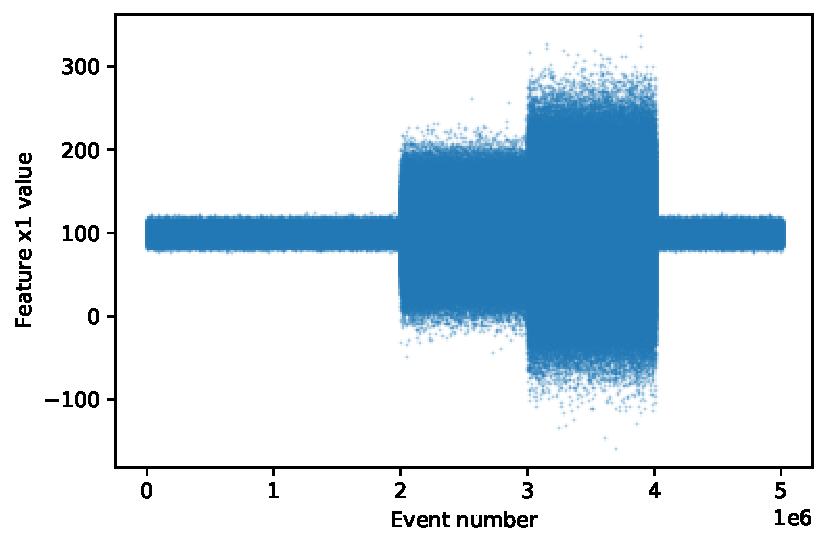
\includegraphics[width=1\linewidth]{figures/timeseries-t4.pdf}
  \captionof{figure}{Time-series for dataset T4}
  \label{fig:timeseries-t4}
\end{minipage}
\end{center}

The reference dataset R4 had a single feature that followed a Gaussian distribution of $\mu=100$ and $\sigma=5$ for all 5 million events. Up until the 2 millionth event, the target dataset T4 followed a Gaussian distribution of $\mu=100$ and $\sigma=5$, similarly to the reference dataset R4. At the 2 millionth event, we change the Gaussian parameters to $\mu=100$ and $\sigma=30$. At the 3 millionth mark, we once again change the Gaussian parameters to $\mu=100$ and $\sigma=50$. Finally, on the 4 millionth event, we return to our reference distribution, a gaussian with $\mu=100$ and $\sigma=5$.


Figure \ref{fig:JSD-signal-test04} shows the computed JSD signal for the target period. As expected, our JSD signal increases at the 2 millionth and 3 millionth event mark, because the distribution parameters change. At the 4 millionth event, we use the original reference distribution and notice that the JSD signal returns to values below the threshold, considering it a normal state, as we intended. Figure \ref{fig:JSD-signal-zoom-test04} is a zoom in on the first 2 millionth events before any change occurs, and we see no false positives.

\begin{figure}[!htb]
\centering
\begin{subfigure}{.5\textwidth}
  \centering
  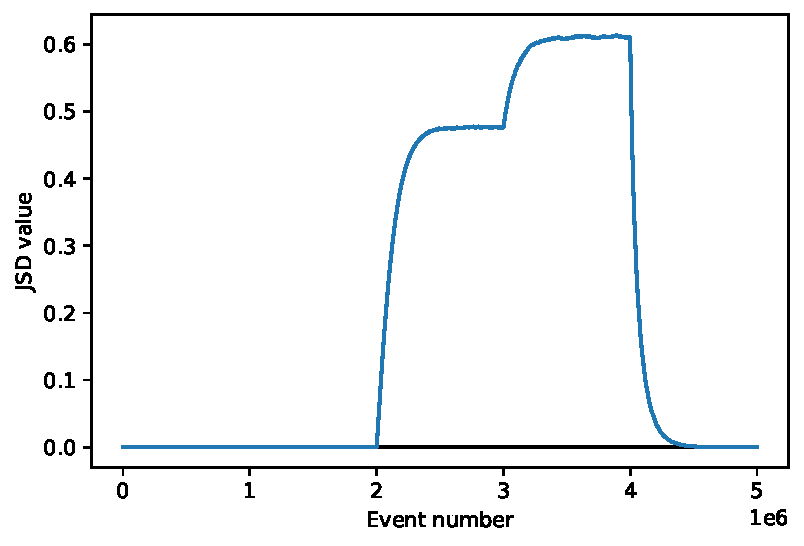
\includegraphics[width=1\linewidth]{figures/stream-analysis-viz-test04.pdf}
  \captionof{figure}{JSD signal and threshold}
  \label{fig:JSD-signal-test04}
\end{subfigure}%
\begin{subfigure}{.5\textwidth}
  \centering
  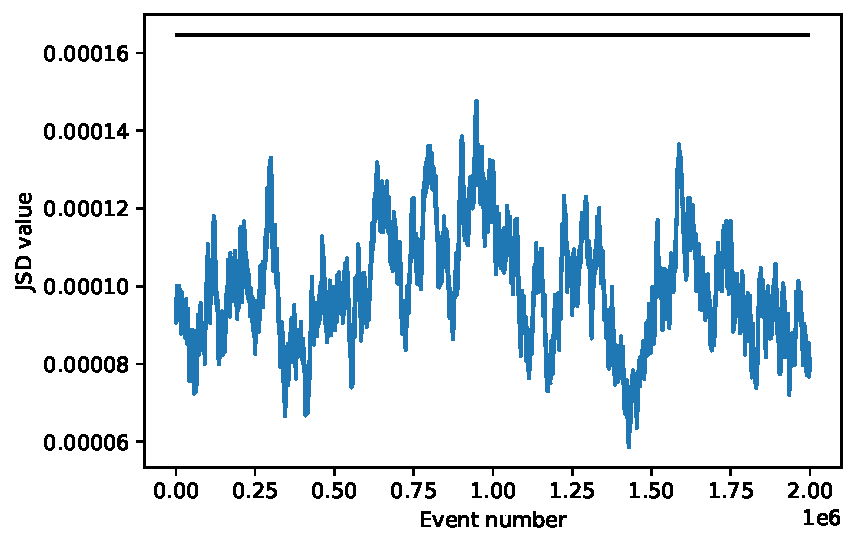
\includegraphics[width=1\linewidth]{figures/stream-analysis-viz-zoom-test04.pdf}
  \caption{Zoom in on the first 2 million events}
  \label{fig:JSD-signal-zoom-test04}
\end{subfigure}
\caption{JSD signal and threshold}
\end{figure}


\subsubsection{An Attempt to Deceive our Method}
In this experiment, we attempt to deceive our method by using a different distribution from the reference period but ensuring its domain is roughly the same as the reference one.

We used the reference dataset R5 (Figure \ref{fig:timeseries-r5}) which had 5 million events, with a single feature that followed a gaussian with  $\mu=100$ and $\sigma=10$. Our target dataset T5 is represented in Figure \ref{fig:timeseries-t5}. For the first 2 million events, the generating distribution used was similar to the one used in the reference dataset, a gaussian with $\mu=100$ and $\sigma=10$. However, at the 2 millionth event, we change the gaussian standard deviation to $\sigma=30$. Then, at the 4 millionth event, we change the distribution type. We use an uniform distribution with lower bound $a=80$ and upper bound $b=120$. Note in Figure \ref{fig:timeseries-t5} that this last portion resembles the first one, the reference.
\begin{center}
\begin{minipage}{.5\textwidth}
  \centering
  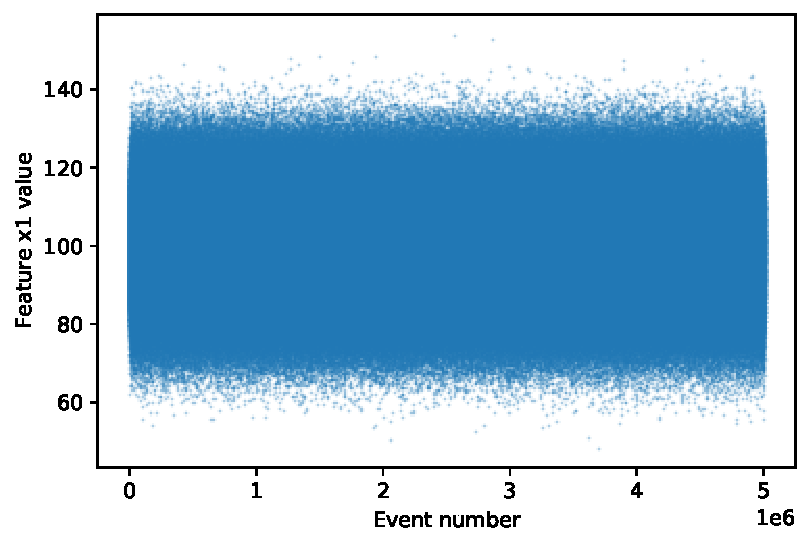
\includegraphics[width=1\linewidth]{figures/timeseries-r5.pdf}
  \captionof{figure}{Time-series for dataset R5}
  \label{fig:timeseries-r5}
\end{minipage}%
\begin{minipage}{.5\textwidth}
  \centering
  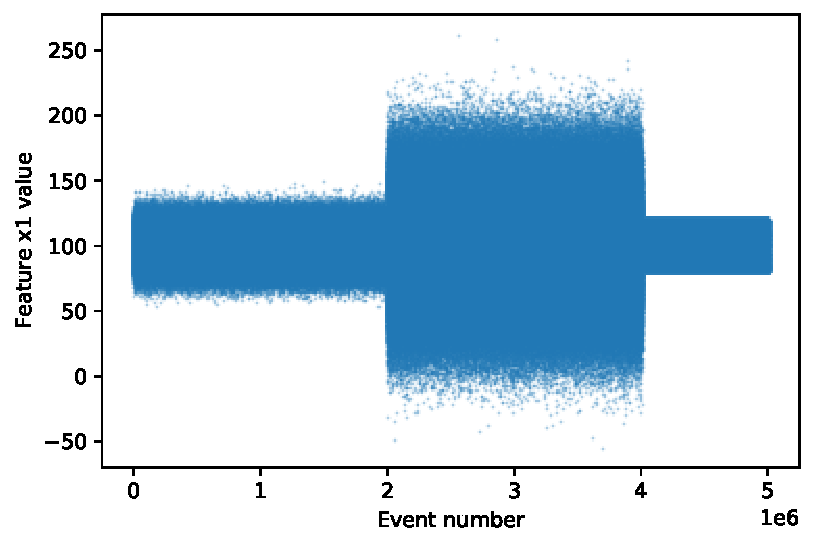
\includegraphics[width=1\linewidth]{figures/timeseries-t5.pdf}
  \captionof{figure}{Time-series for dataset T5}
  \label{fig:timeseries-t5}
\end{minipage}
\end{center}

Let's take a look at the signal computed for the target period. Figure \ref{fig:JSD-signal-test05} shows us the JSD signal for dataset T5 (Figure \ref{fig:timeseries-t5}). As expected, we see a rapid growth of JSD value after the 2 millionth event, when we change the Gaussian parameters. We then change the distribution type, from a gaussian to a uniform one. Despite the latter having a domain contained within the former, we see that our signal is accurate and does not drop below the alert threshold. This is still a different distribution that we want to alert. Figure \ref{fig:JSD-signal-zoom-test05} is a zoom in of the first 2 millionth events and once again we have no false positives.
\begin{figure}[!htb]
\centering
\begin{subfigure}{.5\textwidth}
  \centering
  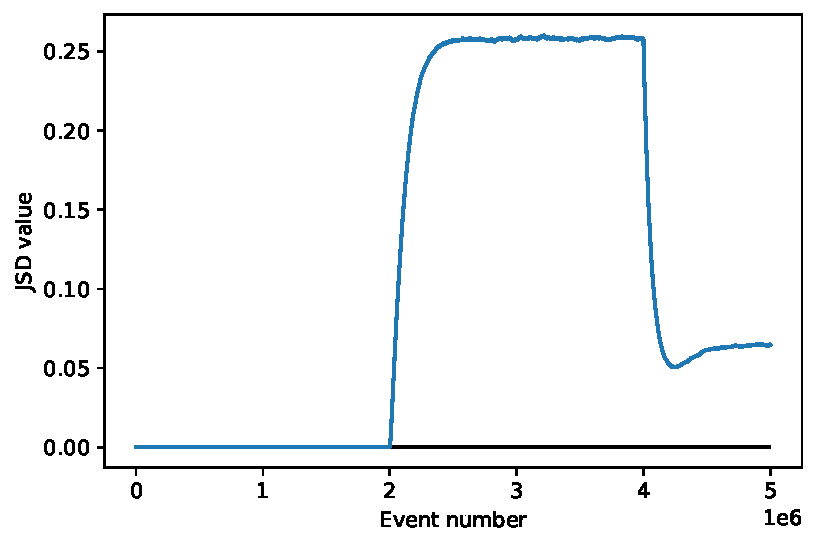
\includegraphics[width=1\linewidth]{figures/stream-analysis-viz-test05.pdf}
  \captionof{figure}{JSD signal and threshold}
  \label{fig:JSD-signal-test05}
\end{subfigure}%
\begin{subfigure}{.5\textwidth}
  \centering
  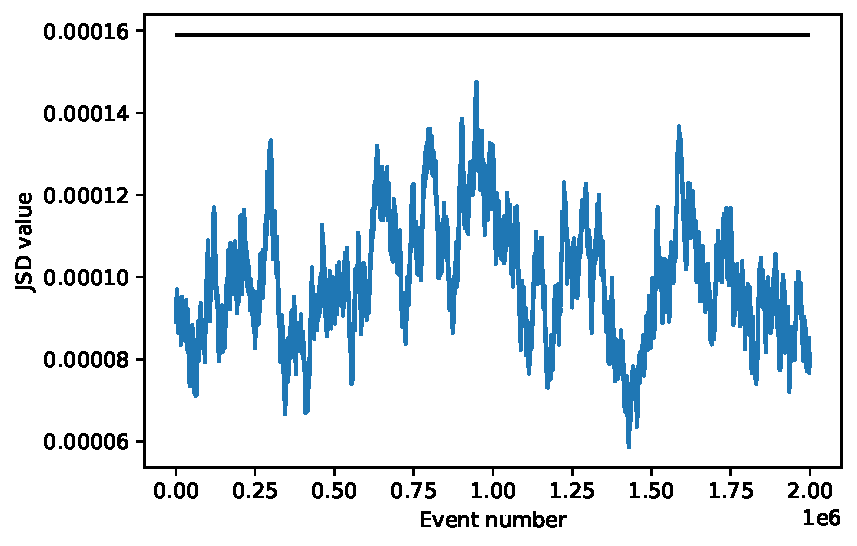
\includegraphics[width=1\linewidth]{figures/stream-analysis-viz-zoom-test05.pdf}
  \caption{Zoom in on the first 2 million events}
  \label{fig:JSD-signal-zoom-test05}
\end{subfigure}
\caption{JSD signal and threshold}
\end{figure}

\subsection{Multi-Feature Analysis}
Before moving to real data, we performed one last experiment, using synthetic data but this time performing a multi-feature analysis. Table \ref{tbl:multi-feat-ref-dataset-distros} shows the underlying generating distributions and parameters for each of the four features ($x_1$, $x_2$, $x_3$ and $x_4$) in the reference multi-feature dataset R6. Figures \ref{fig:timeseries-r6-x1}, \ref{fig:timeseries-r6-x2}, \ref{fig:timeseries-r6-x3} and \ref{fig:timeseries-r6-x4} show the reference time-series for features $x_1$, $x_2$, $x_3$ and $x_4$ on the reference dataset R6, respectively.

\begin{table}[!htb]
    \begin{center}
        \begin{tabular}{|c|c|c|ll}
        \cline{1-3}
        \textbf{Feature} & \textbf{Reference Distribution} & \textbf{Parameters} &  &  \\ \cline{1-3}
        $x_1$               & Gaussian/Normal                 & $\mu=100$, $\sigma=5$  &  &  \\ \cline{1-3}
        $x_2$               & Gaussian/Normal                 & $\mu=100$, $\sigma=5$  &  &  \\ \cline{1-3}
        $x_3$               & Uniform                         & $a=200$, $b=250$       &  &  \\ \cline{1-3}
        $x_4$               & Uniform                         & $a=50$, $b=125$        &  &  \\ \cline{1-3}
        \end{tabular}
    \end{center}
    \caption{Multi-feature reference dataset and feature distributions}
    \label{tbl:multi-feat-ref-dataset-distros}
\end{table}


\begin{figure}[!htb] 
  \begin{minipage}[b]{0.5\linewidth}
    \centering
    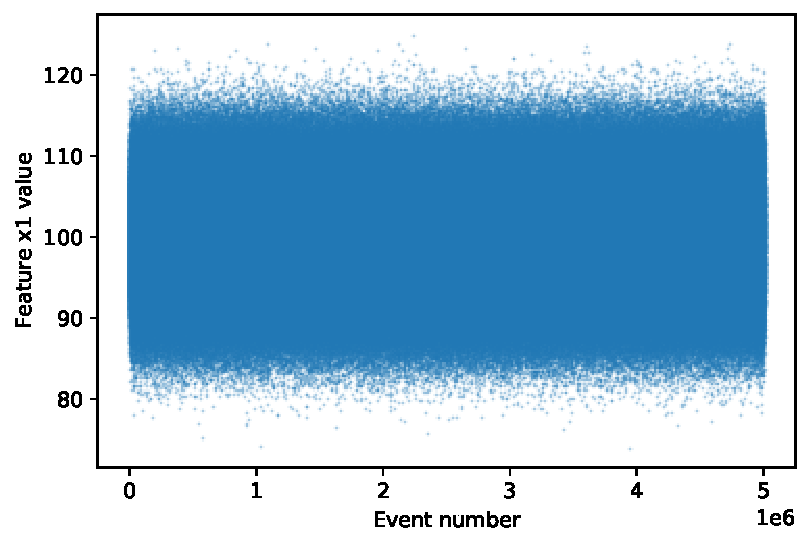
\includegraphics[width=1\linewidth]{figures/timeseries-r6-x1.pdf} 
    \caption{Feature $x_1$ reference time-series} 
    \label{fig:timeseries-r6-x1} 
    \vspace{4ex}
  \end{minipage}%%
  \begin{minipage}[b]{0.5\linewidth}
    \centering
    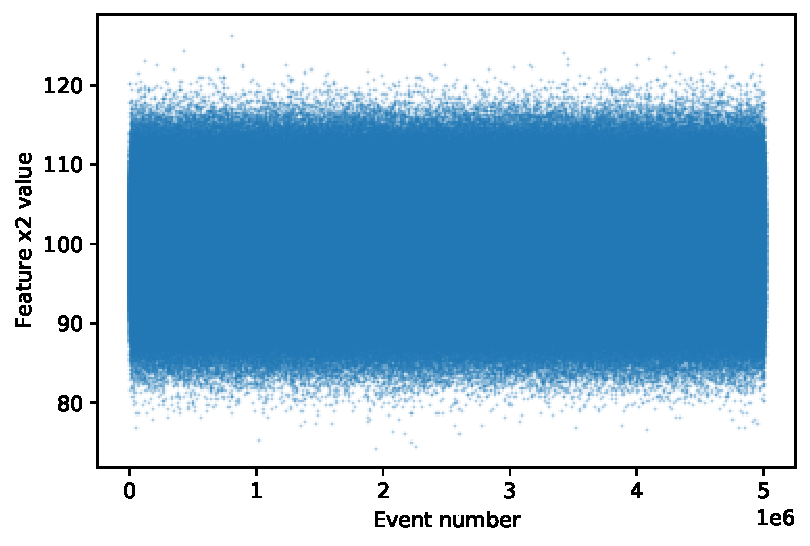
\includegraphics[width=1\linewidth]{figures/timeseries-r6-x2.pdf} 
    \caption{Feature $x_2$ reference time-series} 
    \label{fig:timeseries-r6-x2} 
    \vspace{4ex}
  \end{minipage} 
  \begin{minipage}[b]{0.5\linewidth}
    \centering
    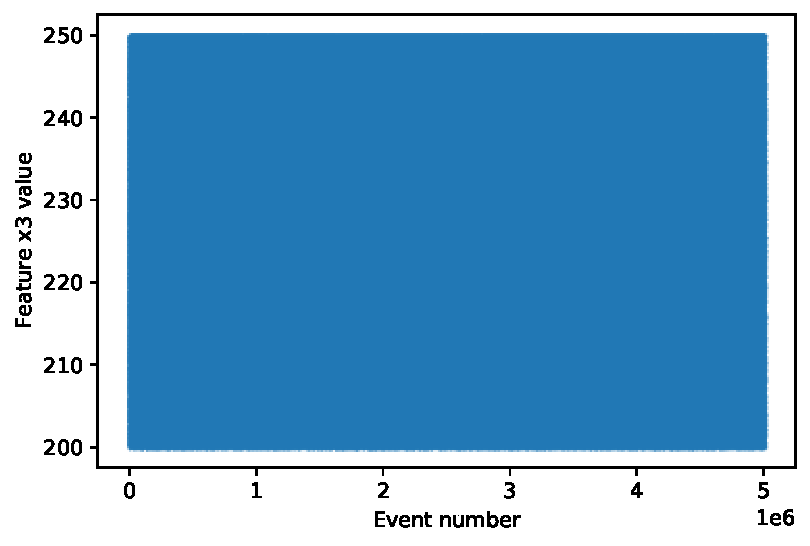
\includegraphics[width=1\linewidth]{figures/timeseries-r6-x3.pdf} 
    \caption{Feature $x_3$ reference time-series} 
    \label{fig:timeseries-r6-x3} 
    \vspace{4ex}
  \end{minipage}%% 
  \begin{minipage}[b]{0.5\linewidth}
    \centering
    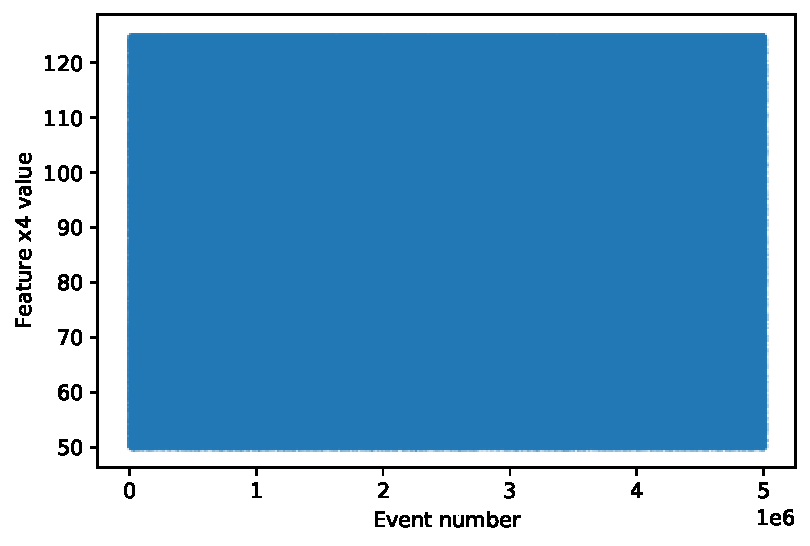
\includegraphics[width=1\linewidth]{figures/timeseries-r6-x4.pdf} 
    \caption{Feature $x_4$ reference time-series} 
    \label{fig:timeseries-r6-x4} 
    \vspace{4ex}
  \end{minipage} 
\end{figure}

We used a target dataset T6 with 5 million events and the same four features ($x_1$, $x_2$, $x_3$ and $x_4$). Feature $x_1$ followed the reference distribution for the 5 million events of the target dataset. We did not change this feature underlying distribution to serve as a control, \textit{i.e.}, we expect no alerts for this one. Figure \ref{fig:timeseries-t6-x1} shows the time-series for the target dataset T6 and feature $x_1$.

Feature $x_2$'s underlying distribution changed four times and returned to normal, so we expect to see alarms with increasing divergence values but eventually no more alarms. Figure \ref{fig:timeseries-t6-x2} shows the time-series for the target dataset T6 and feature $x_2$. Feature $x_2$ followed a gaussian with $\mu=100$ and $\sigma=5$ like in the reference period up to the 1 millionth event mark, then a gaussian with $\mu=100$ and $\sigma=10$ up to the 2.5 millionth event, then a gaussian $\mu=100$ and $\sigma=15$ until the 3 millionth event, then a gaussian $\mu=100$ and $\sigma=20$ until the 4 millionth event and finally returned to the original gaussian with $\mu=100$ and $\sigma=5$ until the last event. Table \ref{tbl:multi-feat-x2-changes} sums up the distributions used and its parameters for each interval of the reference dataset for feature $x_2$.
\begin{table}[!htb]
    \begin{center}
    \begin{tabular}{|c|c|c|c|l}
    \cline{1-4}
    \textbf{From Event} & \textbf{To Event} & \textbf{Distribution} & \multicolumn{1}{l|}{\textbf{Parameters}} &  \\ \cline{1-4}
    0                   & 1,000,000         & Gaussian              & $\mu=100, \sigma=5$                      &  \\ \cline{1-4}
    1,000,000           & 2,500,000         & Gaussian              & $\mu=100, \sigma=10$                     &  \\ \cline{1-4}
    2,500,000           & 3,000,000         & Gaussian              & $\mu=100, \sigma=15$                     &  \\ \cline{1-4}
    3,000,000           & 4,000,000         & Gaussian              & $\mu=100, \sigma=20$                      &  \\ \cline{1-4}
    4,000,000           & 5,000,000         & Gaussian              & $\mu=100, \sigma=5$                      &  \\ \cline{1-4}
    \end{tabular}
    \end{center}
    \caption{Feature $x_2$ generating distributions}
    \label{tbl:multi-feat-x2-changes}
\end{table}

Feature $x_3$'s underlying distribution changed three times and never returned to normal, so we expect to see alarms with increasing divergence values up until the end of the stream analysis. Figure \ref{fig:timeseries-t6-x3} shows the time-series for the target dataset T6 and feature $x_3$. Feature $x_3$ followed a uniform distribution with $a=200$ and $b=250$ like in the reference period up to the 1.5 millionth event mark, then a uniform distribution with $a=200$ and $b=220$ up to the 2 millionth event, then a uniform distribution with $a=180$ and $b=200$ until the 3.5 millionth event and finally a gaussian with $\mu=50$ and $\sigma=20$ until the last event. Table \ref{tbl:multi-feat-x3-changes} sums up the distributions used and its parameters for each interval of the reference dataset for feature $x_3$.
\begin{table}[!htb]
    \begin{center}
    \begin{tabular}{|c|c|c|c|l}
    \cline{1-4}
    \textbf{From Event} & \textbf{To Event} & \textbf{Distribution} & \multicolumn{1}{l|}{\textbf{Parameters}} &  \\ \cline{1-4}
    0                   & 1,500,000         & Uniform               & $a=200, b=250$                           &  \\ \cline{1-4}
    1,500,000           & 2,000,000         & Uniform               & $a=200, b=220$                           &  \\ \cline{1-4}
    2,000,000            & 3,500,000         & Uniform               & $a=180, b=200$                           &  \\ \cline{1-4}
    3,500,000           & 5,000,000         & Gaussian              & $\mu=50, \sigma=20$                      &  \\ \cline{1-4}
    \end{tabular}
    \end{center}
    \caption{Feature $x_3$ generating distributions}
    \label{tbl:multi-feat-x3-changes}
\end{table}

Feature $x_4$'s underlying distribution changed two times and returned to normal, so we expect to see no alarms towards the end of the stream analysis. Figure \ref{fig:timeseries-t6-x4} shows the time-series for the target dataset T6 and feature $x_4$. Feature $x_4$ followed a uniform distribution like the reference one, with $a=50$ and $b=125$ up until the 1.5 millionth event. After that, it followed a uniform distribution with $a=125$ and $b=200$ until the 3 millionth event where it resumed its original uniform distribution (with $a=50$ and $b=125$) until the end. Table \ref{tbl:multi-feat-x4-changes} sums up the distributions used and its parameters for each interval of the reference dataset for feature $x_4$.
\begin{table}[!htb]
    \begin{center}
    \begin{tabular}{|c|c|c|c|l}
    \cline{1-4}
    \textbf{From Event} & \textbf{To Event} & \textbf{Distribution} & \multicolumn{1}{l|}{\textbf{Parameters}} &  \\ \cline{1-4}
    0                   & 1,500,000         & Uniform               & $a=50, b=125$                            &  \\ \cline{1-4}
    1,500,000           & 3,000,000         & Uniform               & $a=125, b=200$                           &  \\ \cline{1-4}
    3,000,000           & 5,000,000         & Uniform               & $a=50, b=125$                            &  \\ \cline{1-4}
    \end{tabular}
    \end{center}
    \caption{Feature $x_4$ generating distributions}
    \label{tbl:multi-feat-x4-changes}
\end{table}


\begin{figure}[!htb] 
  \begin{minipage}[b]{0.5\linewidth}
    \centering
    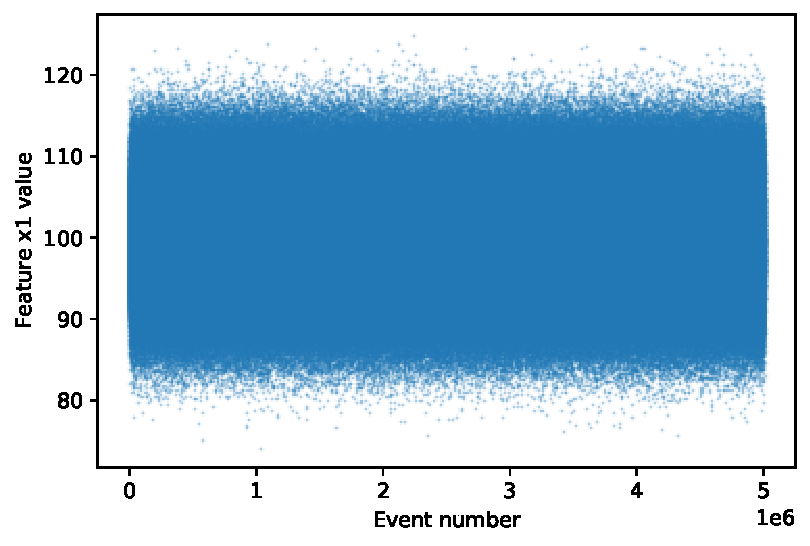
\includegraphics[width=1\linewidth]{figures/timeseries-t6-x1.pdf} 
    \caption{Feature $x_1$ target time-series} 
    \label{fig:timeseries-t6-x1} 
    \vspace{4ex}
  \end{minipage}%%
  \begin{minipage}[b]{0.5\linewidth}
    \centering
    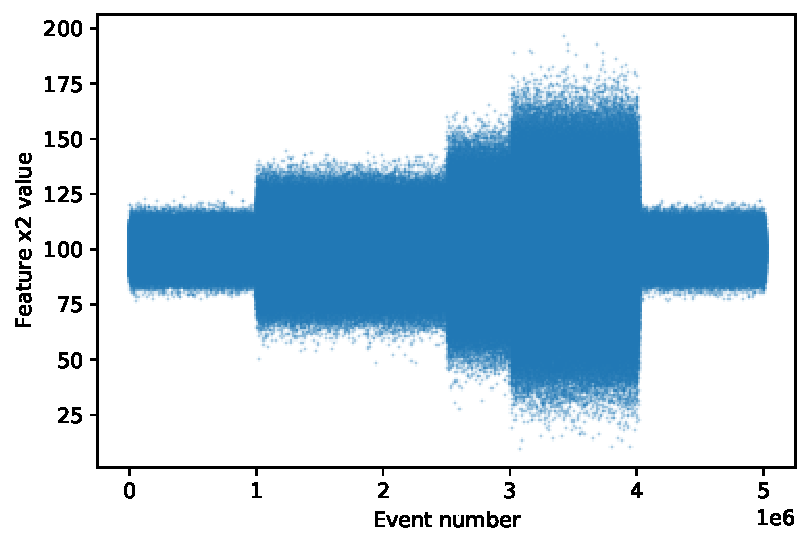
\includegraphics[width=1\linewidth]{figures/timeseries-t6-x2.pdf} 
    \caption{Feature $x_2$ target time-series} 
    \label{fig:timeseries-t6-x2} 
    \vspace{4ex}
  \end{minipage} 
  \begin{minipage}[b]{0.5\linewidth}
    \centering
    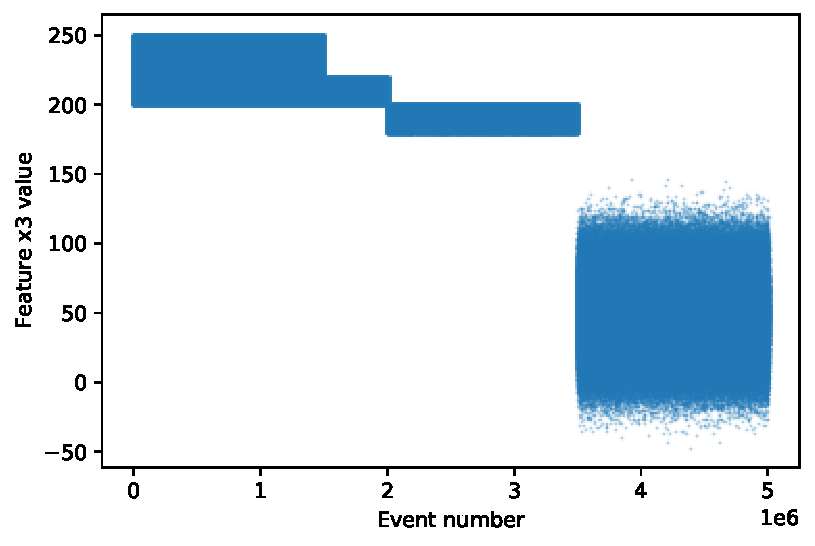
\includegraphics[width=1\linewidth]{figures/timeseries-t6-x3.pdf} 
    \caption{Feature $x_3$ target time-series} 
    \label{fig:timeseries-t6-x3} 
    \vspace{4ex}
  \end{minipage}%% 
  \begin{minipage}[b]{0.5\linewidth}
    \centering
    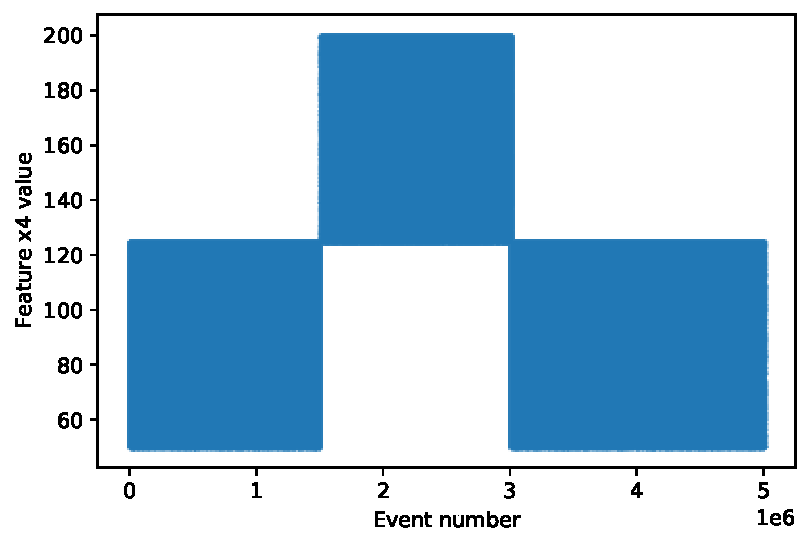
\includegraphics[width=1\linewidth]{figures/timeseries-t6-x4.pdf} 
    \caption{Feature $x_4$ target time-series} 
    \label{fig:timeseries-t6-x4} 
    \vspace{4ex}
  \end{minipage} 
\end{figure}

In this experiment, we used a tuple-based half-life $n_{1/2}=62500$, \textit{i.e.}, sampling and target windows of 250,000 tuples. We used 100 bins for the reference histogram plus the two special infinity bins. In this multi-feature scenario, we used the Holm-Bonferroni correction discussed in Section \ref{sec:holmbonferroni} and set the Family-Wise Error Rate (FWER) to 1\% (FWER = 0.01). Furthermore, instead of doing 1000 samples as we did previously in an ad-hoc way, we use Equation \ref{eq:optimal-n-samples} to determine the minimum number of samples to make while ensuring $\gamma=1\%$ (recall Section \ref{sec:nsamples}). For our four feature analysis scenario, using as inputs  $\gamma=0.01$ and $FWER=0.01$ in Equation \ref{eq:optimal-n-samples} tells us we need to make 1840 samples minimum. Using 300 Spark executors, each given 3G of memory, we finished the batch phase in 418 seconds.

In Section \ref{sec:stream-phase}, we mention that, in our stream analysis, we perform our multiple hypothesis divergence tests on a fixed user-defined frequency. Finding an optimal frequency value for the test falls out of scope for this thesis, but ideally, we set it to be large enough so that we do fewer computations and achieve higher throughput but still get alerts in useful time. In this experiment, we performed the divergence test with the Holm-Bonferroni correction \ref{sec:holmbonferroni} for every new event (frequency of 1 event). We did this to collect a list of ordered corrected p-values for each feature. A corrected p-value (derived from Equation \ref{eq:corrected-pvalue}) is given by:
\begin{equation}
    p-value_{corrected} = p-value_{distance_{x}} * (m - k)
    \label{for:corrected-pvalue}
\end{equation}
With this list, for each feature, we can plot the corrected p-values on each event and compare it with the FWER threshold $\alpha$. Note that despite performing the test at the maximum frequency (in real-time) we still achieved a throughput of 17,921 transactions per second (TPS), even if only for four features.

In the following plots, unlike the JSD signal plots presented before, a feature is in a divergent state if its p-value is below the threshold, according to Equation \ref{eq:corrected-pvalue}. Working with corrected p-values (Formula \ref{for:corrected-pvalue}), a feature is considered divergent if its corrected p-value is below the threshold.

In Figure \ref{fig:x1-corrected-pvalues} we see the plot of corrected p-values for feature $x_1$ and the probability threshold black horizontal line at the bottom. Recall that feature $x_1$'s values were generated by a Gaussian distribution for both the reference period (Figure \ref{fig:timeseries-r6-x1}) and the target period (Figure \ref{fig:timeseries-t6-x1}), with the same parameters. We observe that the corrected p-values never pass below the threshold, as we expected. Hence, this feature is never alerted as divergent.
\begin{figure}[!htb]
    \begin{center}
      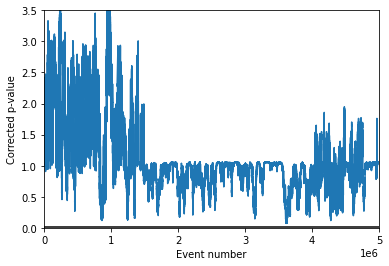
\includegraphics[scale=0.8]{figures/x1-corrected-pvalues.png}
      \caption{Feature $x_1$ corrected p-values and threshold}
      \label{fig:x1-corrected-pvalues}
    \end{center}
\end{figure}

Figure \ref{fig:x2-corrected-pvalues} shows a plot of feature $x_2$'s corrected p-values and the FWER threshold. Feature $x_2$ underlying distribution was changed four times (Table \ref{tbl:multi-feat-x2-changes}): at the 1, 2.5, 3 and 4 millionth events. The first change is consistent with the sudden drop in corrected p-value for this feature, as we cross below the threshold and enter a divergent state. Around a thousand events after the change we saw p-values of 0.2\% (or 0.002). The values keep dropping as time passes and as we introduce bigger changes in distribution.
\begin{figure}[!htb]
    \begin{center}
      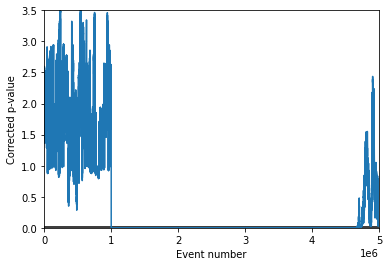
\includegraphics[scale=0.8]{figures/x2-corrected-pvalues.png}
      \caption{Feature $x_2$ corrected p-values and threshold}
      \label{fig:x2-corrected-pvalues}
    \end{center}
\end{figure}
We resume the reference or original distribution at the 4 millionth event. However, as we can see from a close-up on the original plot (Figure \ref{fig:x2-corrected-pvalues-zoom}), it takes around 600,000 events for the target sliding histogram aggregation to once again resemble the reference one, resulting in a high enough p-value and thus stop alerting $x_2$ as divergent.
\begin{figure}[!htb]
    \begin{center}
      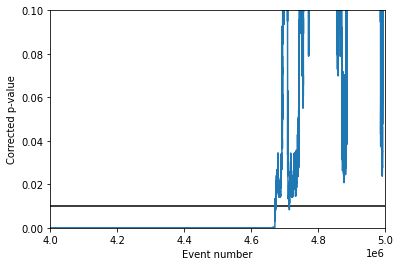
\includegraphics[scale=0.8]{figures/x2-corrected-pvalues-zoom2.png}
      \caption{Feature $x_2$ zoomed in corrected p-values and threshold}
      \label{fig:x2-corrected-pvalues-zoom}
    \end{center}
\end{figure}


Feature $x_3$ was the only feature that never returned to its original distribution and is the only one that should be reported until the end as divergent. This is in fact the case as illustrated in Figure \ref{fig:x3-corrected-pvalues}. The first change to $x_3$'s generating distribution was introduced at the 1.5 millionth event and we clearly see the corrected p-value rapidly approaching values close to zero. For the rest of the dataset, this $x_3$'s p-value remains below the threshold, as we never swap to its original distribution.
\begin{figure}[!htb]
    \begin{center}
      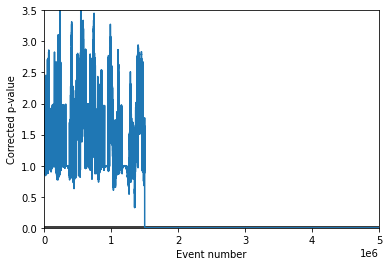
\includegraphics[scale=0.8]{figures/x3-corrected-pvalues.png}
      \caption{Feature $x_3$ corrected p-values and threshold}
      \label{fig:x3-corrected-pvalues}
    \end{center}
\end{figure}


Finally, feature $x_4$'s corrected p-value plot is given by Figure \ref{fig:x4-corrected-pvalues}. Similarly to feature $x_2$, we resume the original distribution at a certain point, in this case at the 3-millionth event. However, as we can see from a close-up on the original plot (Figure \ref{fig:x4-corrected-pvalues-zoom}), it takes around 810,000 events for the target sliding window aggregation to be considered similar enough to the reference one and stop alerting $x_4$ as divergent.
\begin{figure}[!htb]
    \begin{center}
      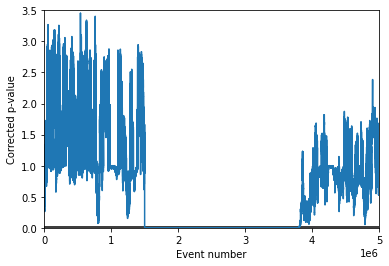
\includegraphics[scale=0.8]{figures/x4-corrected-pvalues.png}
      \caption{Feature $x_4$ corrected p-values and threshold}
      \label{fig:x4-corrected-pvalues}
    \end{center}
\end{figure}
\begin{figure}[!htb]
    \begin{center}
      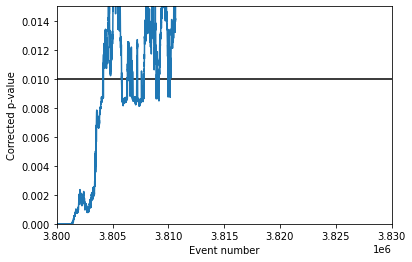
\includegraphics[scale=0.8]{figures/x4-corrected-pvalues-zoom2.png}
      \caption{Feature $x_4$ zoomed in corrected p-values and threshold}
      \label{fig:x4-corrected-pvalues-zoom}
    \end{center}
\end{figure}


With this experiment, we further validate that the p-value is a measure of how divergent a feature is: the closer to zero, the lower the probability of the statistical test result and hence the more divergent a feature is considered to be. At the 1.5 millionth event, we swap both $x_3$ and $x_4$'s distribution. For the first 2,535,000 events, $x_4$ has a lower p-value than $x_3$ and hence is considered more divergent. However, after that, we change $x_3$'s distribution so aggressively that $x_3$ starts being reported as most divergent, with a lower p-value than $x_4$.

\clearpage
\section{Experiments with Real Data}

Due to time constraints, we experimented with data from only one merchant. The merchant's entity as well as feature names will remain anonymous due to confidentiality reasons.

Feedzai provides a fraud detection solution for this merchant and had stored two contiguous in time datasets of credit card transactions that, combined, covered a period of roughly 1 year and 9 months. In this experiment, we used the older one as the reference dataset and the more recent one as the target period. Both datasets were already feature-engineered \cite{Domingos-ML-Feat-Eng} and had a total of 183 numerical plus numerically encoded categorical features (\textit{e.g.}, one-hot encoded or ordinal encoded \cite{categoricalencoding}). Table \ref{tbl:merchant1-datasets-summary} shows summary statistics for both datasets.
\begin{table}[!htb]
    \begin{center}
        \begin{tabular}{|c|c|c|c|}
        \hline
        \textbf{Dataset} & \textbf{From}              & \textbf{To}           & \multicolumn{1}{l|}{\textbf{Transactions}} \\ \hline
        Reference        & Tuesday, September 5, 2017 & Friday, June 29, 2018 & 1,604,509                                  \\ \hline
        Target           & Friday, June 29, 2018      & Sunday, June 30, 2019 & 4,032,505                                  \\ \hline
        \end{tabular}
        \caption{Summary statistics for reference and target merchant datasets}
        \label{tbl:merchant1-datasets-summary}
    \end{center}
\end{table}

In the batch phase, we used 100 Spark executors, each with 12G of memory. We determined that one week's worth of data for this merchant was on average equivalent to 37,803 events. We set the half-life to be $n_{1/2}=37,803$ and discard events whose EMA weight is 6\% or less, which is equivalent to using sampling windows of data of four times the half-life (as detailed in Section \ref{sec:ema-hist}). Hence, our samples's windows had 151,212 events. Using Equation \ref{eq:optimal-n-samples}, we determined that for 183 features, a FWER of 1\% and $\gamma$ (as defined in Section \ref{sec:nsamples}) of 10\% we needed to make a minimum of 42,137 samples. Our batch analysis took 5 hours and 34 minutes.

After the batch phase, we had the necessary inputs for the streaming phase (detailed in Section \ref{sec:batch-artifacts-summary}), namely, for each feature, the reference histograms, the list of observed divergence values and the last sample's histogram. We then used the target dataset, simulating a stream of ordered events. Our monitoring system processed the dataset event by event in sequential, time-ordered fashion, emulating a stream computation and reported divergent features with associated p-values. We performed our multiple hypotheses with the Holm-Bonferroni correction (Section \ref{sec:holmbonferroni}) for every 1000 events. It took us 382,363 milliseconds (roughly 6 minutes) to process the 4,032,505 transactions, amounting to a throughput of 10,546 transactions per second (TPS).

This merchant and in particular these datasets were known to suffer a lot from concept drift. Our system produced a large list of alerts, from nearly the beginning of the target period until the end. Due to a large number of features (183), we only show some plots. Furthermore, we refer to features with anonymized identifiers, like feature $x_j$. In the following plots, we show the corrected p-values (Formula \ref{for:corrected-pvalue}) for some features at each event of the time-series and the FWER threshold set at 1\%. A feature is considered divergent at a given timestamp if below that threshold line.

Figure \ref{fig:merchant-x1-reference} is a plot of the reference time-series of feature $x_1$ and Figure \ref{fig:merchant-x1-target} the corresponding target time-series.
\begin{figure}[!htb]
    \begin{center}
      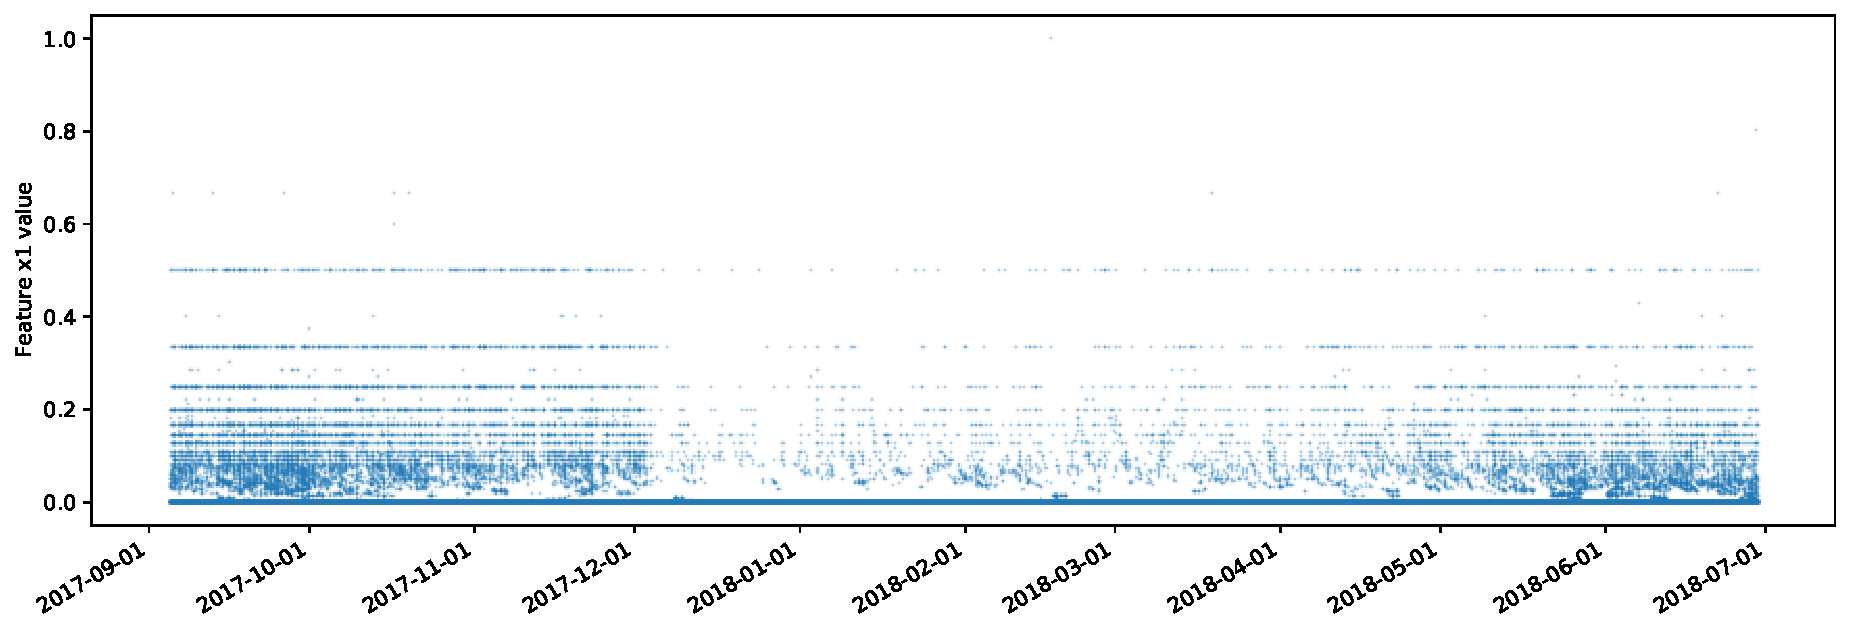
\includegraphics[scale=0.5]{figures/merchant-x1-reference.pdf}
      \caption{Merchant feature $x_1$ reference time-series}
      \label{fig:merchant-x1-reference}
    \end{center}
\end{figure}
\begin{figure}[!htb]
    \begin{center}
      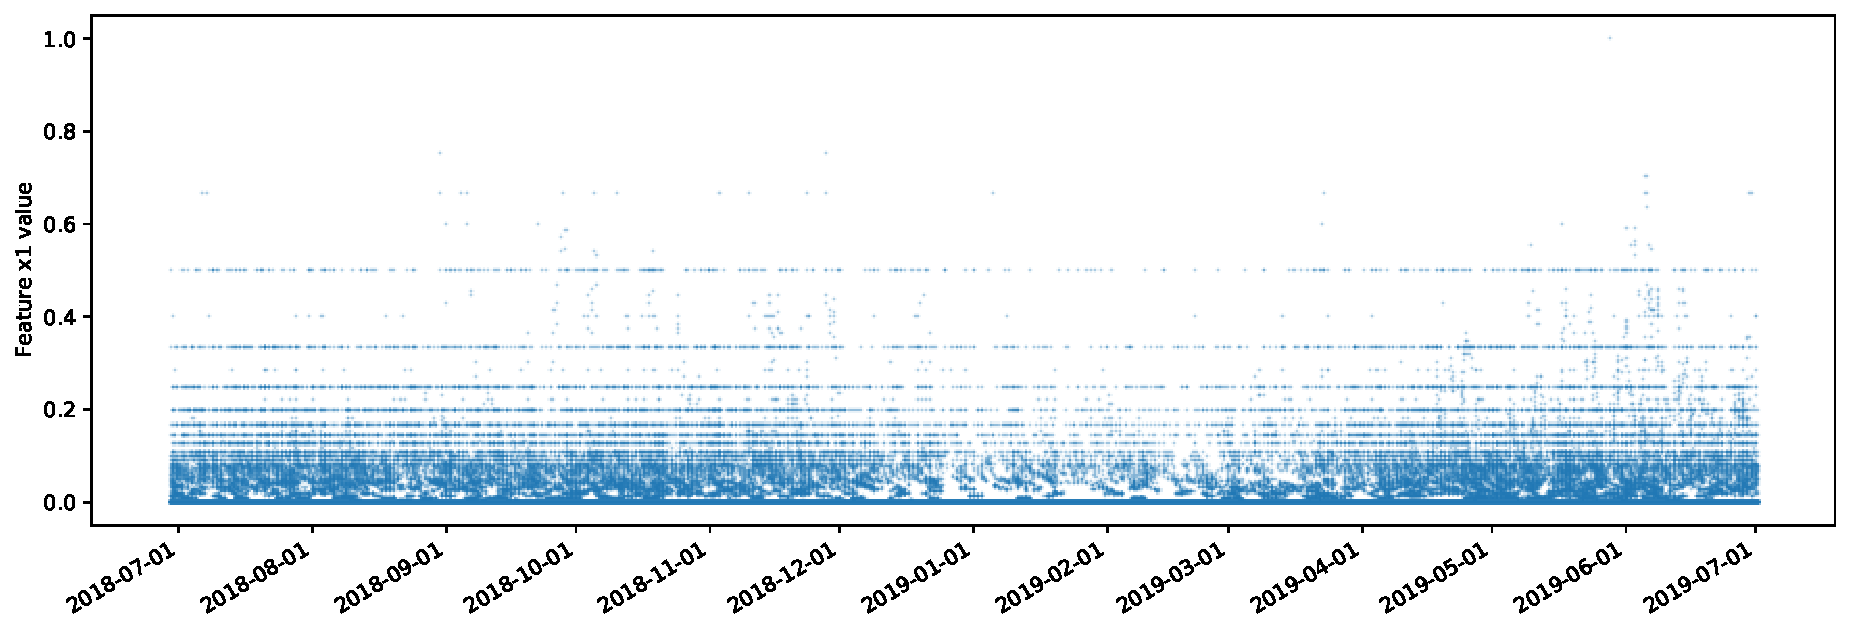
\includegraphics[scale=0.5]{figures/merchant-x1-target.pdf}
      \caption{Merchant feature $x_1$ target time-series}
      \label{fig:merchant-x1-target}
    \end{center}
\end{figure}
In Figure \ref{fig:merchant-x1-correctedpvalues} we plot the corrected p-values for the each event of the target period. The reference and target periods look very similar and in fact we have very few alarms for this feature, \textit{i.e.}, the number of times the line crosses to the bottom half of the plot, imposed by the threshold line. 
\begin{figure}[!htb]
    \begin{center}
      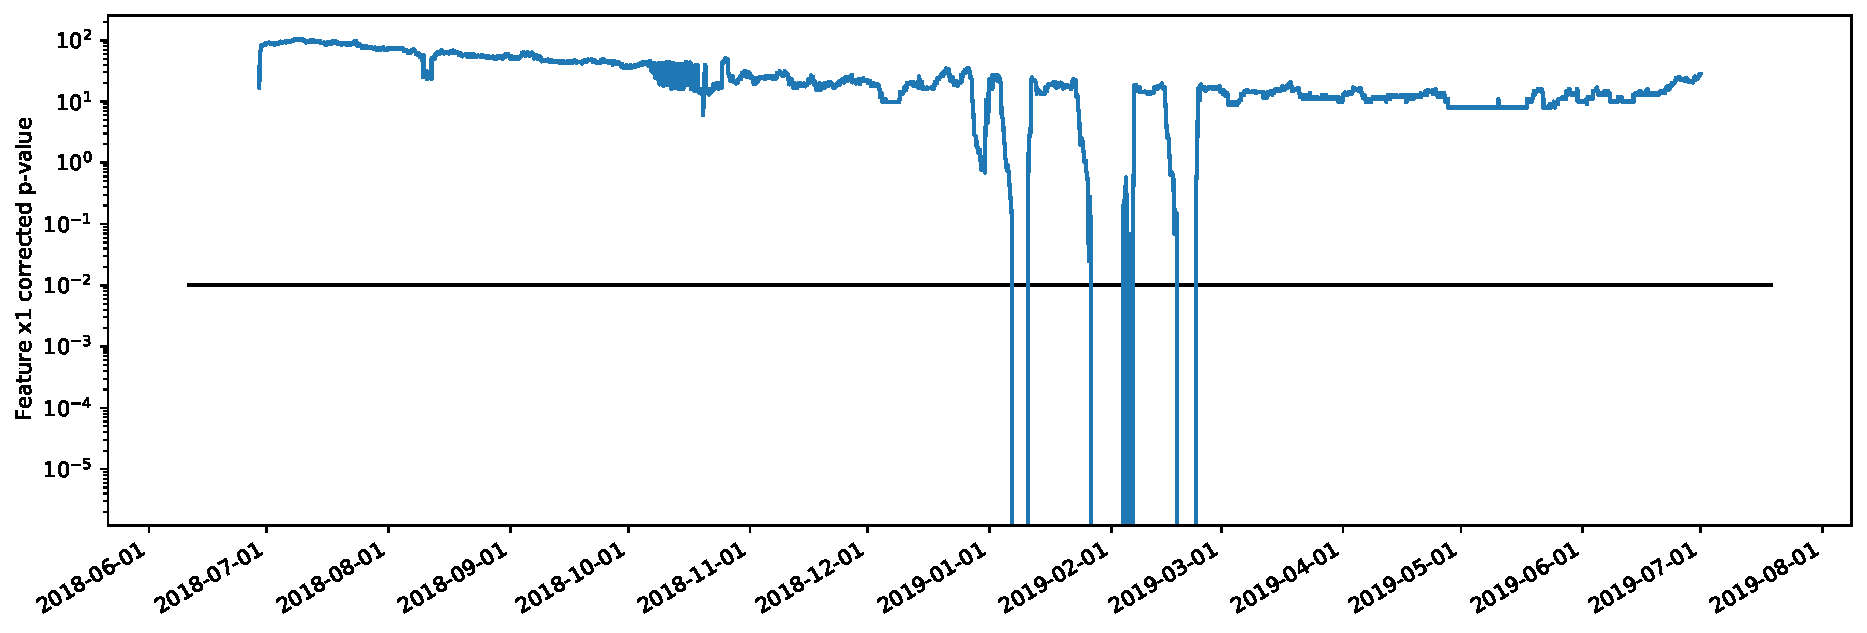
\includegraphics[scale=0.5]{figures/merchant-x1-correctedpvalues.pdf}
      \caption{Merchant feature $x_1$ corrected p-values}
      \label{fig:merchant-x1-correctedpvalues}
    \end{center}
\end{figure}
Furthermore, the alarms appear to be roughly in the middle portion of the time-series, where in fact the target period appears to have less points. We can see roughly three alarms. The first one in early January 2019 for a few days, the second one lasting about a week at the end of January 2019 and the last one in the second half of February 2019 again for a few days.

Now let us look at features $x_2$ and $x_3$. Figures \ref{fig:merchant-x2-reference} and \ref{fig:merchant-x2-target} show feature $x_2$'s time-series plots for the reference and target periods, respectively.
\begin{figure}[!htb]
    \begin{center}
      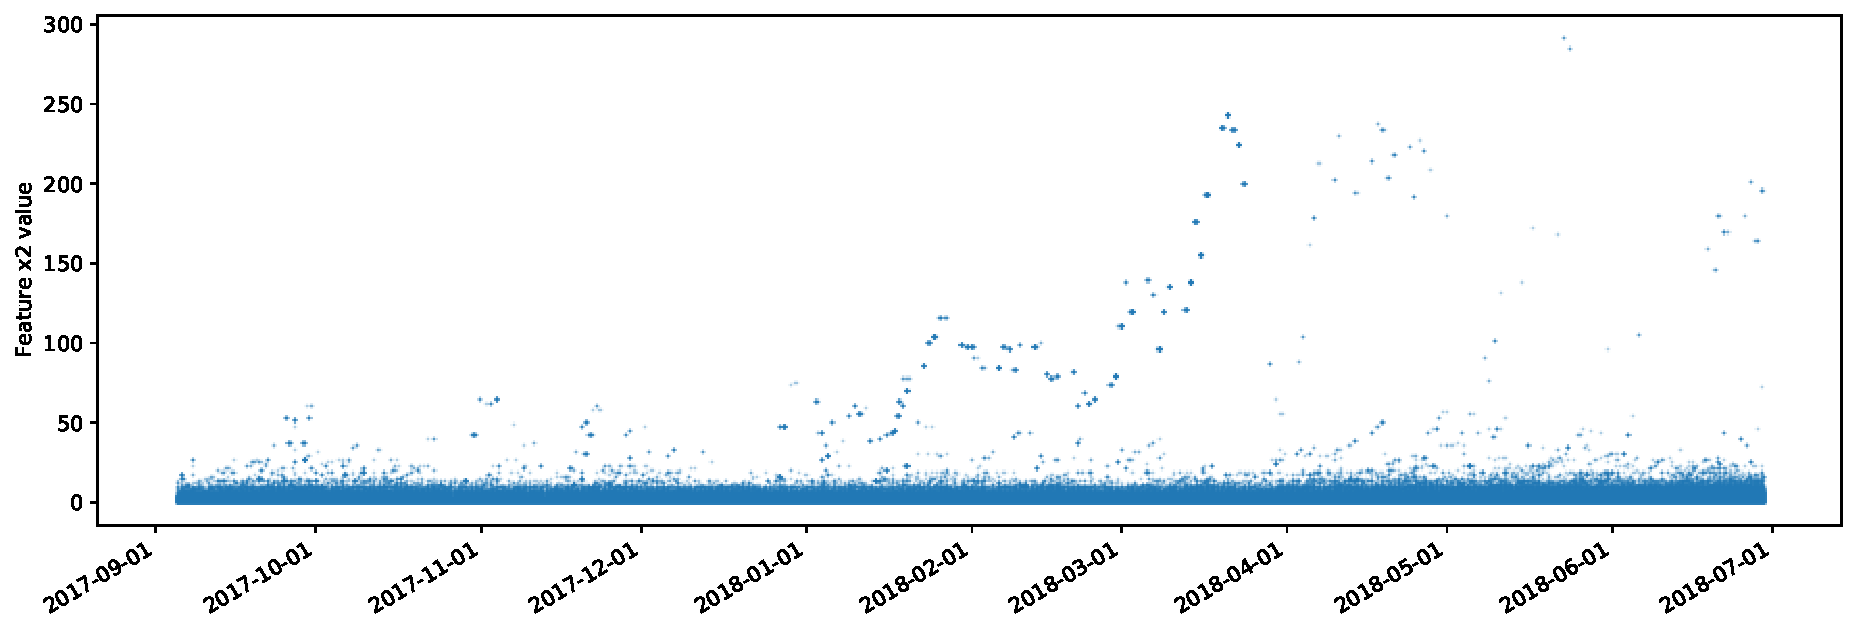
\includegraphics[scale=0.5]{figures/merchant-x2-reference.pdf}
      \caption{Merchant feature $x_2$ reference time-series}
      \label{fig:merchant-x2-reference}
    \end{center}
\end{figure}
\begin{figure}[!htb]
    \begin{center}
      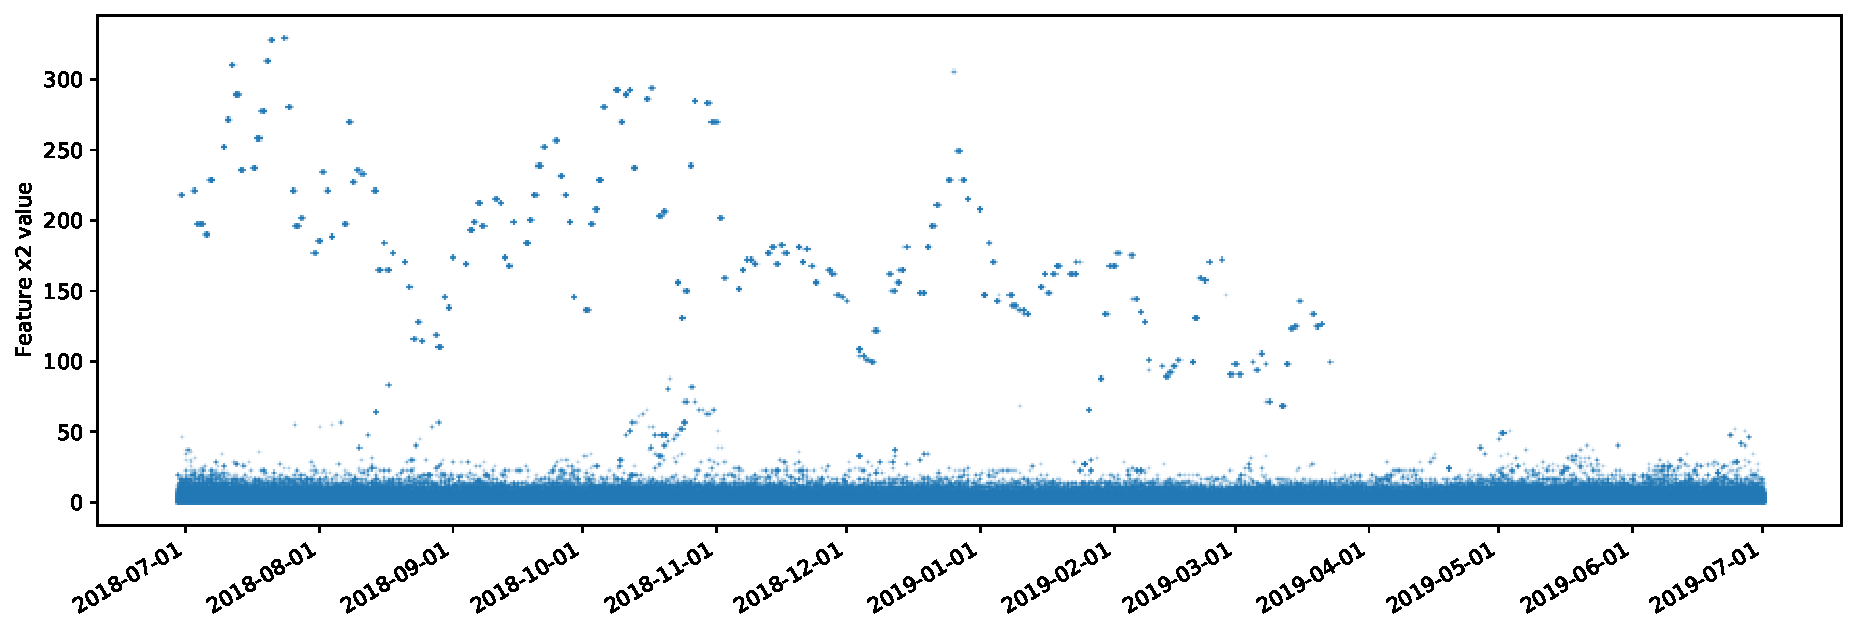
\includegraphics[scale=0.5]{figures/merchant-x2-target.pdf}
      \caption{Merchant feature $x_2$ target time-series}
      \label{fig:merchant-x2-target}
    \end{center}
\end{figure}
Figures \ref{fig:merchant-x3-reference} and \ref{fig:merchant-x3-target} show feature $x_3$'s time-series plots for the reference and target periods, respectively.
\begin{figure}[!htb]
    \begin{center}
      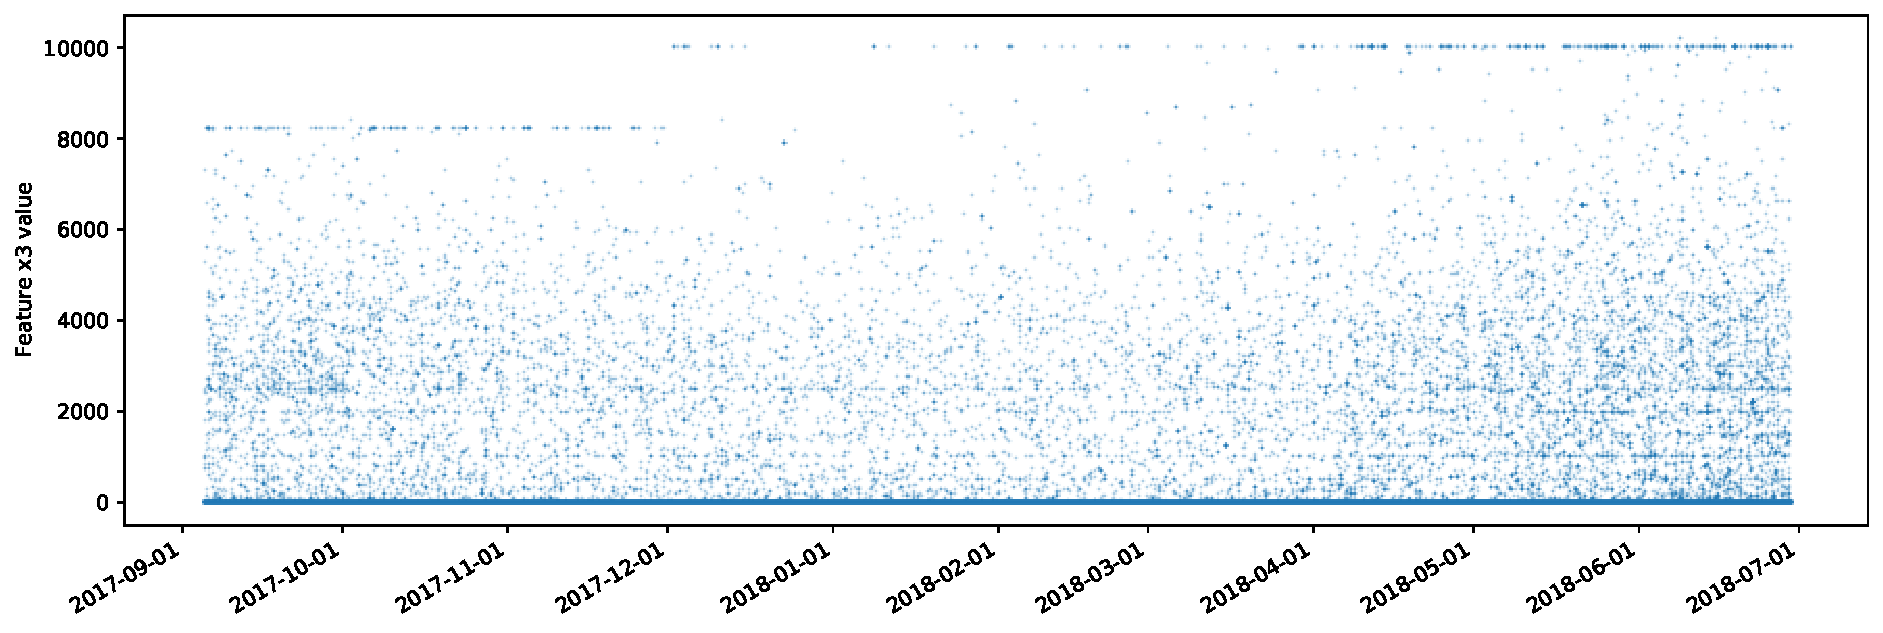
\includegraphics[scale=0.5]{figures/merchant-x3-reference.pdf}
      \caption{Merchant feature $x_3$ reference time-series}
      \label{fig:merchant-x3-reference}
    \end{center}
\end{figure}
\begin{figure}[!htb]
    \begin{center}
      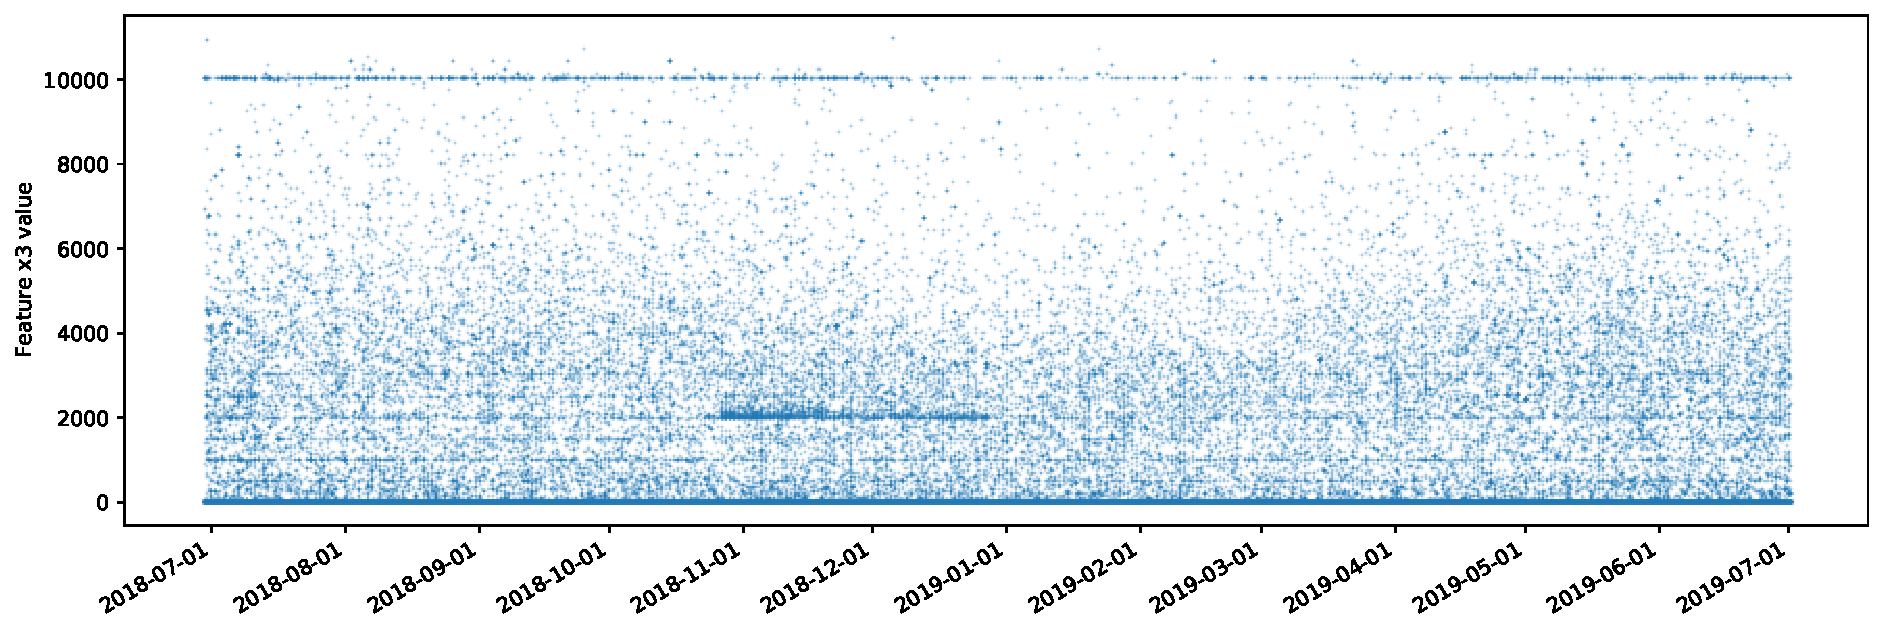
\includegraphics[scale=0.5]{figures/merchant-x3-target.pdf}
      \caption{Merchant feature $x_3$ target time-series}
      \label{fig:merchant-x3-target}
    \end{center}
\end{figure}
\clearpage
Relative to $x_1$, features $x_2$ and $x_3$ also have very similar reference and target periods. Just like feature $x_1$, we expect to have some alarms but still not too many. Once again, to visualize the alarms, we plot the corrected p-values for each event of the target time-series for each feature. Figure \ref{fig:merchant-x2-correctedpvalues} is a plot of feature $x_2$'s corrected p-values and the FWER threshold of 1\%. Likewise, Figure \ref{fig:merchant-x3-correctedpvalues} shows the same plot but for feature $x_3$.
\begin{figure}[!htb]
    \begin{center}
      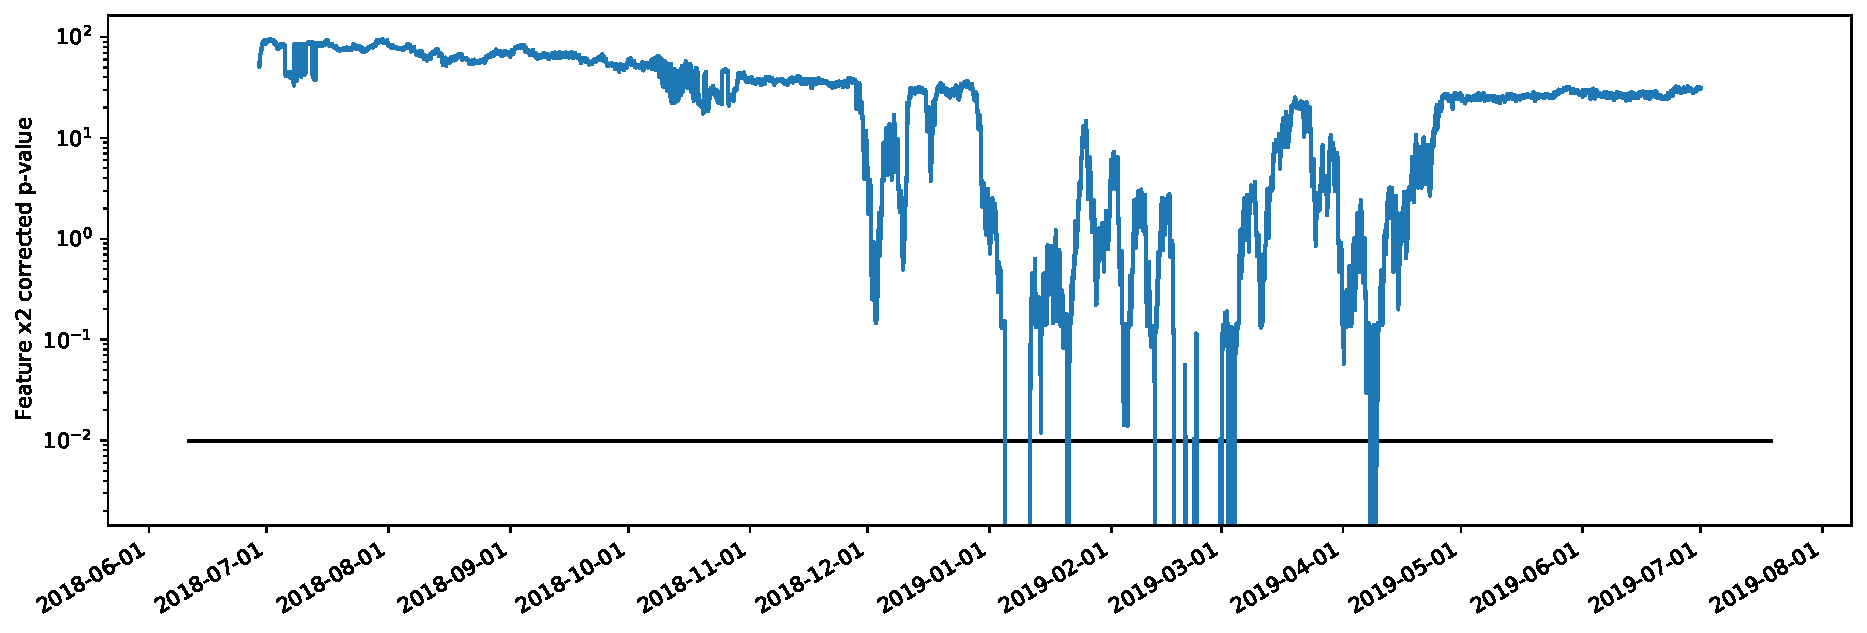
\includegraphics[scale=0.5]{figures/merchant-x2-correctedpvalues.pdf}
      \caption{Merchant feature $x_2$ corrected p-values}
      \label{fig:merchant-x2-correctedpvalues}
    \end{center}
\end{figure}
\begin{figure}[!htb]
    \begin{center}
      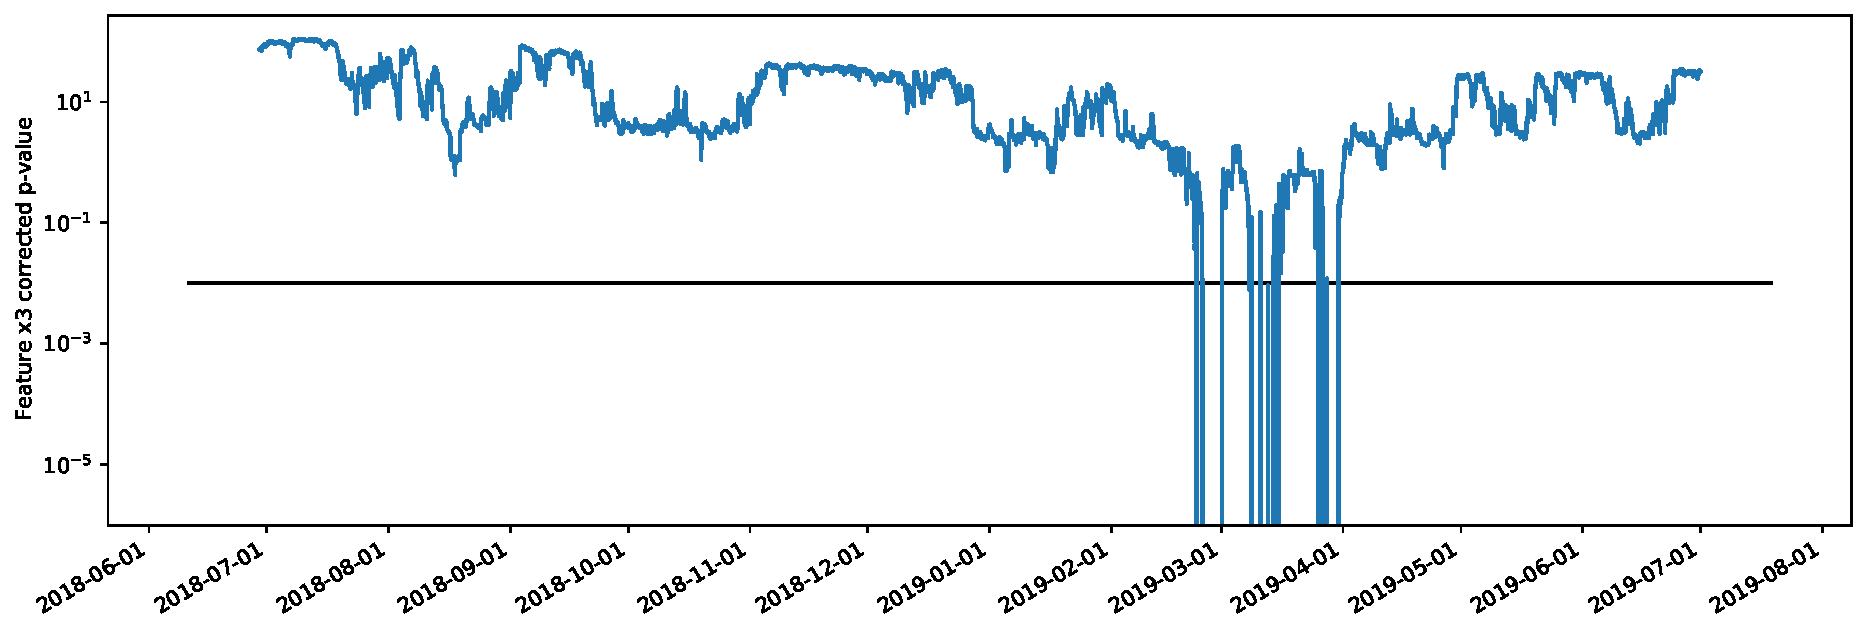
\includegraphics[scale=0.5]{figures/merchant-x3-correctedpvalues.pdf}
      \caption{Merchant feature $x_3$ corrected p-values}
      \label{fig:merchant-x3-correctedpvalues}
    \end{center}
\end{figure}
The corrected p-values plot shows us once again that both $x_2$ and $x_3$ features had some alarms but eventually rose above the threshold and resumed their reference distribution. This is expected from features whose reference and target time-series plots look so similar.

Next, we analyze a feature with very different reference and target time-series. Feature $x_4$'s reference time-series is presented in Figure \ref{fig:merchant-x4-reference} and its target period in Figure \ref{fig:merchant-x4-target}.
\begin{figure}[!htb]
    \begin{center}
      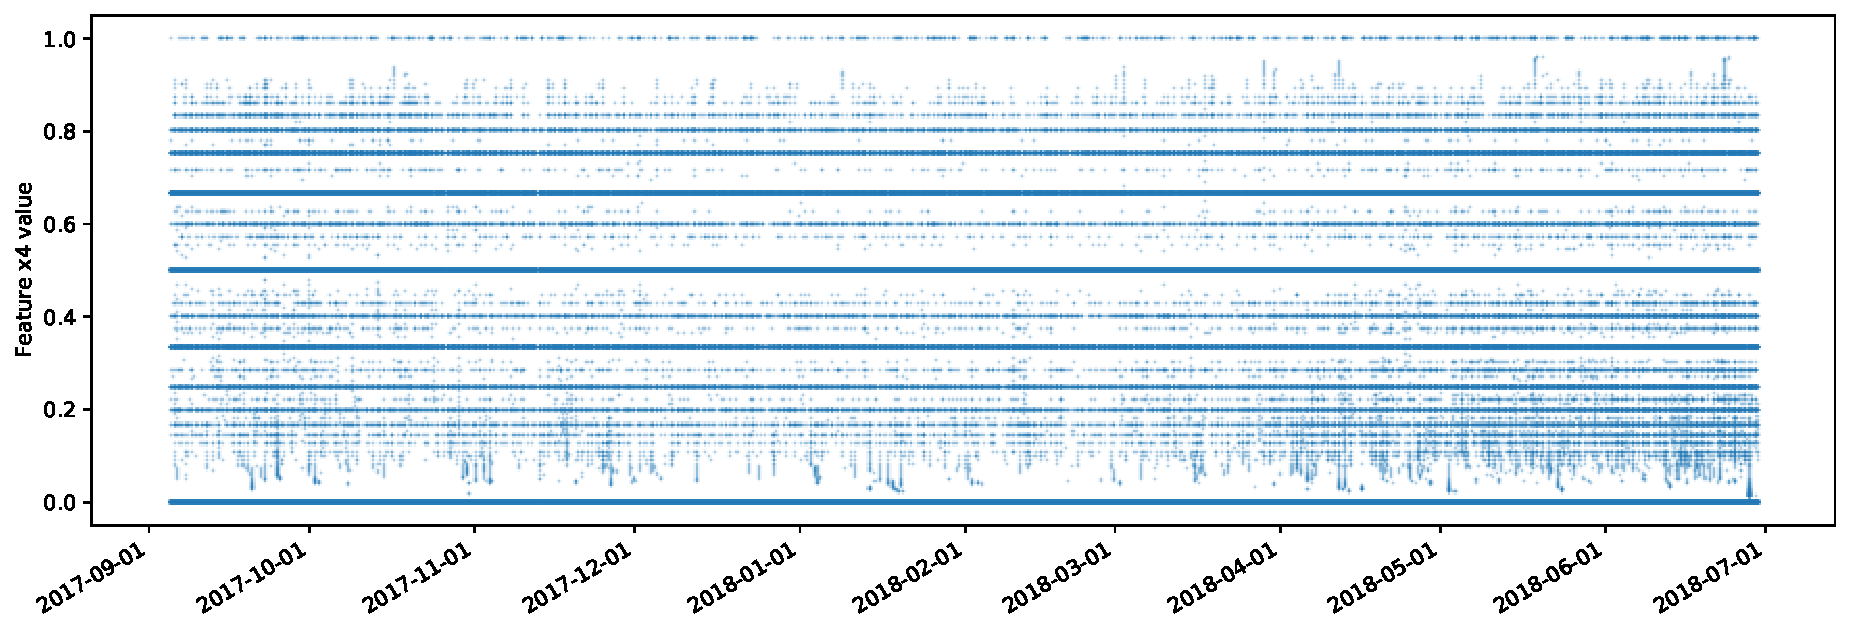
\includegraphics[scale=0.5]{figures/merchant-x4-reference.pdf}
      \caption{Merchant feature $x_4$ reference time-series}
      \label{fig:merchant-x4-reference}
    \end{center}
\end{figure}
\begin{figure}[!htb]
    \begin{center}
      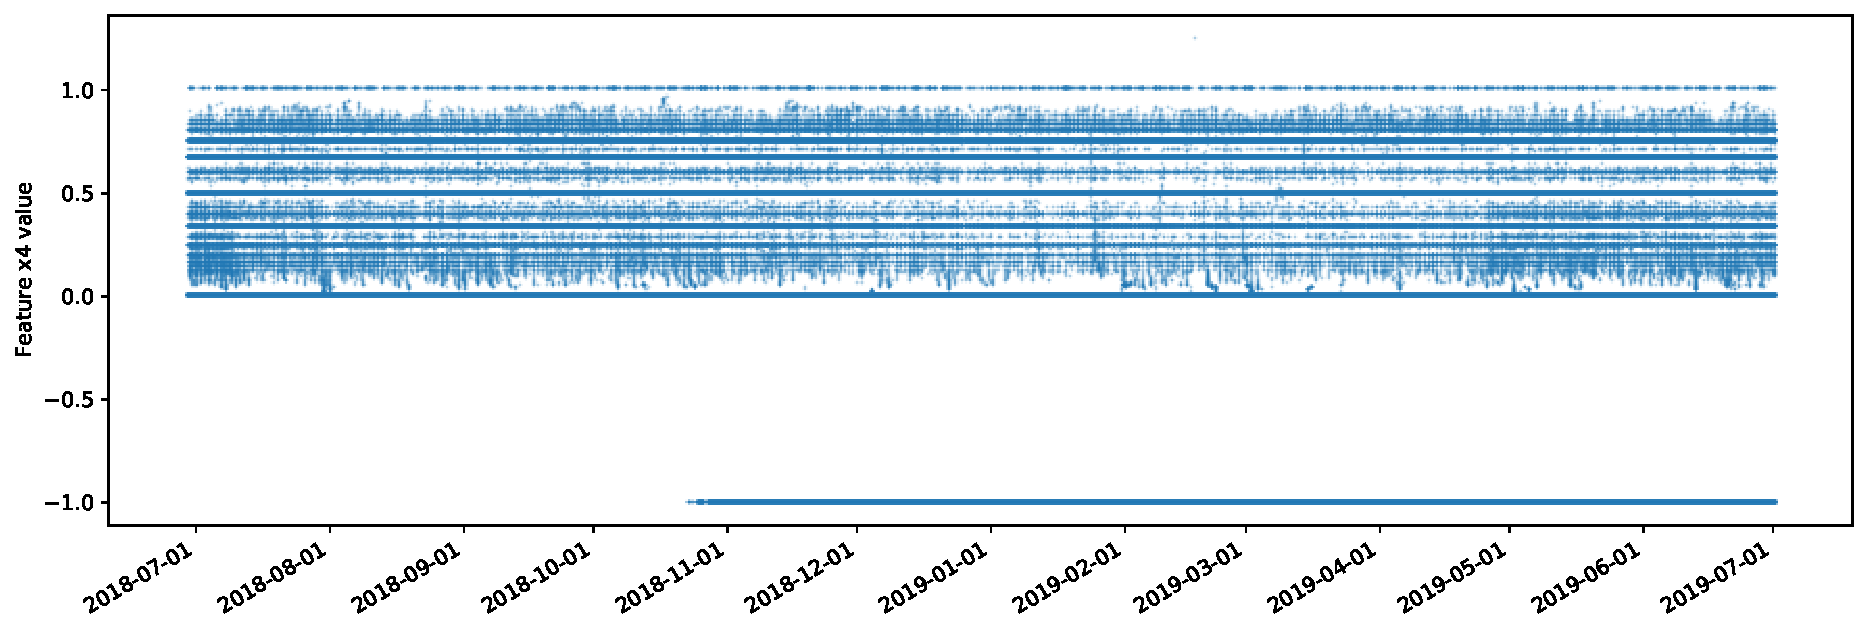
\includegraphics[scale=0.5]{figures/merchant-x4-target.pdf}
      \caption{Merchant feature $x_4$ target time-series}
      \label{fig:merchant-x4-target}
    \end{center}
\end{figure}
Notice that even if for the most part both reference and target periods values belong to a domain between 0 and 1, at a certain point in time, in the target time-series, a lot of -1 values appear. In Figure \ref{fig:merchant-x4-correctedpvalues} we plot the corrected p-values for feature $x_4$ target time-series.
\begin{figure}[!htb]
    \begin{center}
      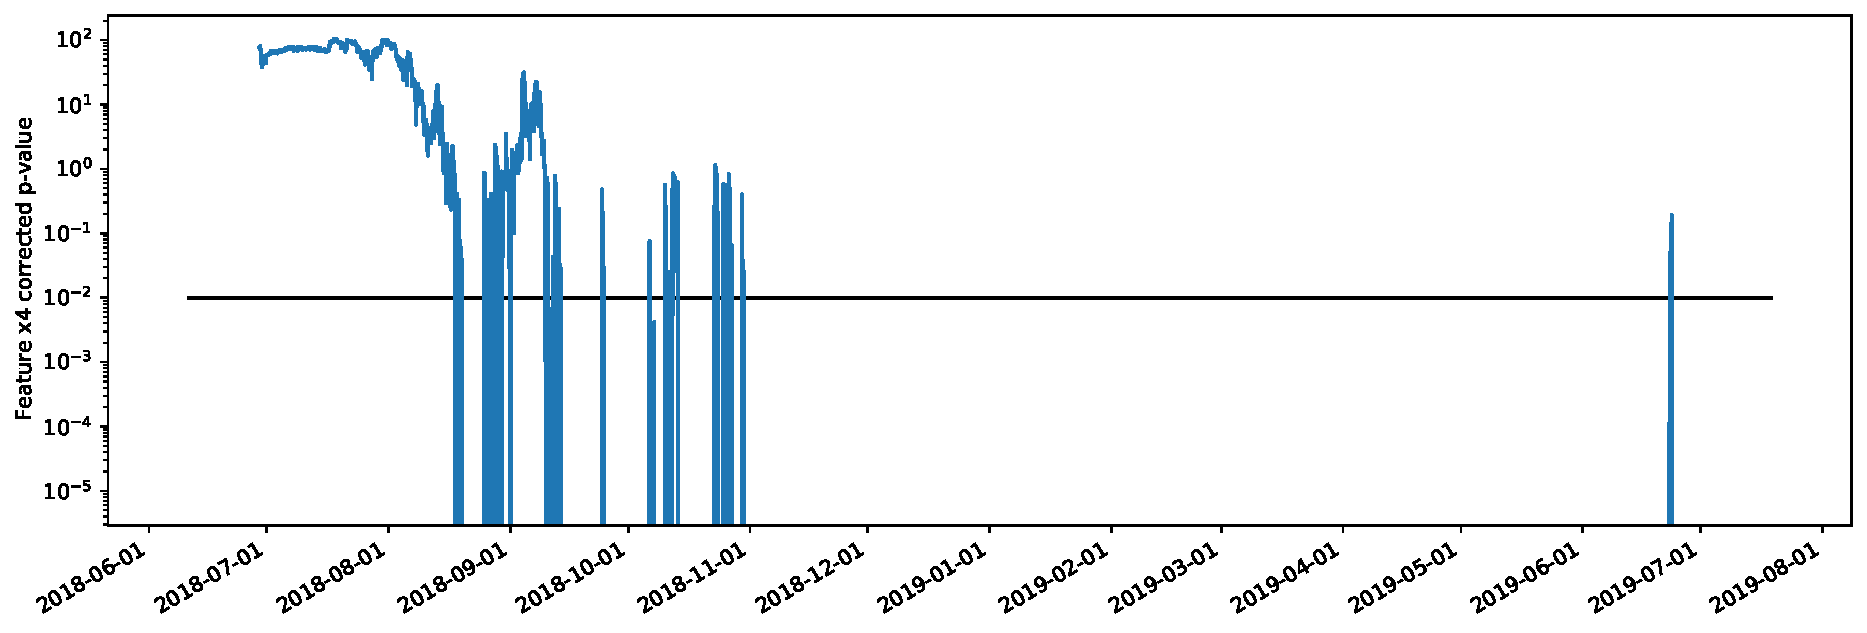
\includegraphics[scale=0.5]{figures/merchant-x4-correctedpvalues.pdf}
      \caption{Merchant feature $x_4$ corrected p-values}
      \label{fig:merchant-x4-correctedpvalues}
    \end{center}
\end{figure}
Like the previous analyzed features, $x_4$ also drops below the threshold some times. However, unlike the other features, where feature values return to normal and alarms stopped being raised, $x_4$ remains below the threshold line until the end of the target period, where a small spike occurs. The last time feature $x_4$ was ever above the threshold line (and hence considered normal) was before the appearance of the -1 values in the target period. This seems to work as expected: -1 values were so off the reference domain that for here on out, as long as these values keep appearing, we will not stop reporting $x_4$ as divergent.

The -1 value is often used as a placeholder for missing values, \textit{i.e.}, if some problem occurs and the value for a feature is missing at a given timestamp or event, -1 is used. A follow-up question that is raised is if we should include some mechanism of dealing with missing values in our method. However, we discard this idea and defend that we should not: missing values are indeed something we want to detect. For instance, if a certain device responsible for reporting one feature stops working, we want to know that. This scenario is likely to happen in a distributed Internet-of-Things (IoT) system with hundreds of devices transmitting data. 

%feats = [max_amt_rate_per_location_72h, num_preauths_per_card_1w, user_avg_amount_completions_1h, completions_rate_per_location_zip3_72h, completion_rate_per_card_72h]
%low drift:
    %x1 - max_amt_rate_per_location_72h
    %x2 - num_preauths_per_card_1w
    %x3 - user_avg_amount_completions_1h
%high drift:
    %x4 - completion_rate_per_card_72h
    %x5 - dif_last_and_current_trx
\subsection{Same Reference and Target Periods}
In this experiment, we set out to test our system in a low drift scenario. To guarantee the reference and target periods are as similar as possible, we decided to use the same dataset to work as reference and target. We chose to use the reference dataset from the previous experiment (Reference of Table \ref{tbl:merchant1-datasets-summary}) and feed it as input for both our batch and stream analysis as the reference and target periods, respectively. We expect to have less alarms for each feature but not necessarily zero.

We first show the corrected p-value plots when both reference and target periods are the same, for the previous features $x_1$, $x_2$ and $x_3$ in Figures \ref{fig:merchant2-x1-correctedpvalues}, \ref{fig:merchant2-x2-correctedpvalues} and \ref{fig:merchant2-x3-correctedpvalues}, respectively. 

Feature $x_1$ has less alerts in this experiment where we use equal reference and target periods. However, the alarms last for about two months. This is unexpected as we predicted we would see no alarms or few ones with short duration. Likewise, we observe that for feature $x_2$ (Figure \ref{fig:merchant2-x2-correctedpvalues}) and $x_3$ (Figure \ref{fig:merchant2-x3-correctedpvalues}) we still have many alarms and some lasting up to one month.
\begin{figure}[!htb]
    \begin{center}
      \includegraphics[scale=0.5]{figures/merchant2-x1-correctedpvalues.pdf}
      \caption{Merchant feature $x_1$ corrected p-values with equal reference and target periods}
      \label{fig:merchant2-x1-correctedpvalues}
    \end{center}
\end{figure}
\begin{figure}[!htb]
    \begin{center}
      \includegraphics[scale=0.5]{figures/merchant2-x2-correctedpvalues.pdf}
      \caption{Merchant feature $x_2$ corrected p-values with equal reference and target periods}
      \label{fig:merchant2-x2-correctedpvalues}
    \end{center}
\end{figure}
\begin{figure}[!htb]
    \begin{center}
      \includegraphics[scale=0.5]{figures/merchant2-x3-correctedpvalues.pdf}
      \caption{Merchant feature $x_3$ corrected p-values with equal reference and target periods}
      \label{fig:merchant2-x3-correctedpvalues}
    \end{center}
\end{figure}
We do not have a clear explanation for this and due to time constraints we leave further tests to future work. We suspect the issue may be that there is a difference between the batch and streaming phases. In batch we have subsets of events and compute EMA-like histogram aggregations based on those. In streaming, however, we have a continuous stream of data and never expire the 6\% of data that in batch is not present, because it is a finite window.

Now we analyze feature $x_4$ from the previous experiment, as this one was the one with the highest measured drift. Recall that feature $x_4$'s target time-series (Figure \ref{fig:merchant-x4-target}) was significantly different from the reference one (Figure \ref{fig:merchant-x4-reference}). Because of this, the corrected p-values plot from the previous experiment (Figure \ref{fig:merchant-x4-correctedpvalues}) crossed our threshold line multiple times and remained in an alert state for most of the target time-series. In this new experiment, we used the reference period twice. Because of this, the corrected p-values plot is now different. Figure \ref{fig:merchant2-x4-correctedpvalues} shows the corrected p-values plot for feature $x_4$ when we used the reference period for both phases.
\begin{figure}[!htb]
    \begin{center}
      \includegraphics[scale=0.5]{figures/merchant2-x4-correctedpvalues.pdf}
      \caption{Merchant feature $x_4$ corrected p-values with equal reference and target periods}
      \label{fig:merchant2-x4-correctedpvalues}
    \end{center}
\end{figure}
Using the same period twice theoretically means we have no drift at all. Hence, we expected to see no alerts. Figure \ref{fig:merchant2-x4-correctedpvalues} shows that we have a few alerts but significantly less than in Figure \ref{fig:merchant-x4-correctedpvalues}. Furthermore, in this new experiment, $x_4$ eventually stops being reported at all until the end of the dataset and ends at a high p-value. Recall that the higher the p-value the less divergent a feature is. Overall, we see that this feature has fewer alarms and stabilizes well above our alarm threshold which is coherent since we used the same dataset as reference and target periods.

We now introduce a new feature, $x_5$. Feature $x_5$ also suffers from a large amount of drift. In the reference and target datasets presented in Table \ref{tbl:merchant1-datasets-summary}, feature $x_5$ reference time-series plot is given by Figure \ref{fig:merchant-x5-reference} and the target time-series by Figure \ref{fig:merchant-x5-target}.
\begin{figure}[!htb]
    \begin{center}
      \includegraphics[scale=0.5]{figures/merchant-x5-reference.pdf}
      \caption{Merchant feature $x_5$ reference time-series}
      \label{fig:merchant-x5-reference}
    \end{center}
\end{figure}
\begin{figure}[!htb]
    \begin{center}
      \includegraphics[scale=0.5]{figures/merchant-x5-target.pdf}
      \caption{Merchant feature $x_5$ target time-series}
      \label{fig:merchant-x5-target}
    \end{center}
\end{figure}
The density in the upper domain of values is clearly different in both reference and target periods. Hence, in our first experiment, this feature had a corrected p-values plot with two alarm states, where the second one lasted until the end of the target period, with the lowest possible p-value (zero), represented in Figure \ref{fig:merchant-x5-correctedpvalues}.
\begin{figure}[!htb]
    \begin{center}
      \includegraphics[scale=0.5]{figures/merchant-x5-correctedpvalues.pdf}
      \caption{Merchant feature $x_5$ corrected p-values}
      \label{fig:merchant-x5-correctedpvalues}
    \end{center}
\end{figure}

However, when using the same reference and target periods, in this case using the time-series in Figure \ref{fig:merchant-x5-reference} twice, we achieve our lowest possible drift scenario. The difference in corrected p-values is clear. Figure \ref{fig:merchant2-x5-correctedpvalues} shows this plot when using equal reference and target periods. We observe that our corrected p-values never go below the threshold line, in fact, they stay well above it. This is expected behavior when using equal reference and target periods.
\begin{figure}[!htb]
    \begin{center}
      \includegraphics[scale=0.5]{figures/merchant2-x5-correctedpvalues.pdf}
      \caption{Merchant feature $x_5$ corrected p-values with equal reference and target periods}
      \label{fig:merchant2-x5-correctedpvalues}
    \end{center}
\end{figure}


\subsection{Building an Accurate Divergence Measure Distribution}
Our method comprises two-phases: the batch and the streaming analysis. We can not conclude in which phase an error that could possibly explain the last experiment's results exists. To isolate both phases, we conduct this last experiment where instead of using the distribution of divergence measures built in the batch phase we use a distribution we know to be the best fit for the streaming period. 

Our best fit divergence distribution was built over the streaming period. To do this, we processed the streaming events once and saved all the JSD measures. We binned these JSD values with 50,000 bins all with equal heights (or counts). Then we performed once again the streaming analysis over the same period but this time using the previously built distribution for which we know it is the best possible fit, since it was computed over the exact same period, built event by event. We set the FWER to be 1\% so we expect to see some alarms, \textit{i.e.}, for JSD measures above the 99th percentile.

Recall that in the last experiment, for feature $x_1$, using the same target and reference periods, we had two large alarms that lasted months (Figure \ref{fig:merchant2-x1-correctedpvalues}). Using the same periods but with the newly computed distribution of divergence measures we obtain the corrected p-values plot shown in Figure \ref{fig:merchant3-x1-correctedpvalues}.
\begin{figure}[!htb]
    \begin{center}
      \includegraphics[scale=0.5]{figures/merchant3-x1-correctedpvalues.pdf}
      \caption{Merchant feature $x_1$ corrected p-values with equal reference and target periods and using the best-fit divergence distribution}
      \label{fig:merchant3-x1-correctedpvalues}
    \end{center}
\end{figure}
This plot actually makes sense and represents expected behavior. Notice that we have only a few short-lasting alarms, which correspond to the JSD measures above the 99th percentile. These can be thought of as false positives. In reality, the definition of the multi-test we perform is exactly this: alert events above the 99th percentile (FWER=1\%).

Figures \ref{fig:merchant3-x2-correctedpvalues}, \ref{fig:merchant3-x3-correctedpvalues}, \ref{fig:merchant3-x4-correctedpvalues} and \ref{fig:merchant3-x5-correctedpvalues} show the corrected p-value plots for this experiment for features $x_2$, $x_3$, $x_4$ and $x_5$, respectively.
\begin{figure}[!htb]
    \begin{center}
      \includegraphics[scale=0.5]{figures/merchant3-x2-correctedpvalues.pdf}
      \caption{Merchant feature $x_2$ corrected p-values with equal reference and target periods and using the best-fit divergence distribution}
      \label{fig:merchant3-x2-correctedpvalues}
    \end{center}
\end{figure}
\begin{figure}[!htb]
    \begin{center}
      \includegraphics[scale=0.5]{figures/merchant3-x3-correctedpvalues.pdf}
      \caption{Merchant feature $x_3$ corrected p-values with equal reference and target periods and using the best-fit divergence distribution}
      \label{fig:merchant3-x3-correctedpvalues}
    \end{center}
\end{figure}
\begin{figure}[!htb]
    \begin{center}
      \includegraphics[scale=0.5]{figures/merchant3-x4-correctedpvalues.pdf}
      \caption{Merchant feature $x_4$ corrected p-values with equal reference and target periods and using the best-fit divergence distribution}
      \label{fig:merchant3-x4-correctedpvalues}
    \end{center}
\end{figure}
\begin{figure}[!htb]
    \begin{center}
      \includegraphics[scale=0.5]{figures/merchant3-x5-correctedpvalues.pdf}
      \caption{Merchant feature $x_5$ corrected p-values with equal reference and target periods and using the best-fit divergence distribution}
      \label{fig:merchant3-x5-correctedpvalues}
    \end{center}
\end{figure}
The analysis performed for feature $x_1$ applies for all of these features. Notice that for all plots we have very few alarms of very short durations. This coherency in results across multiple features seems to indicate that our streaming analysis is accurate and detects the outliers accurately if the divergence measure distribution used is well built.

\newpage
\section{Conclusions}
In this section, we summarize our experimental tests, results and uncovered issues.

We began by performing single-feature analysis of synthetic data. The results obtained with this set of experiments were what we expected, in the sense that the artificially introduced anomalies in the datasets were all correctly reported. Still working with synthetic data, we performed our first multi-feature analysis. In this scenario, we applied the Holm-Bonferroni multiple test correction to the p-values of each hypothesis. Once again, each feature was correctly reported as divergent at the timestamps where we changed the underlying generating distribution.

We then moved on to real data. Due to time constraints and the scope of this thesis, we experimented only with data from one merchant. In our first experiment with real data, we ran our method with what we thought was an ideal set of parameters and produced a lot of alarms. A close analysis of the reference and target time-series of each feature revealed that some alarms indeed made sense, as this dataset contained a lot of drift. 

In our second experiment with real data, we attempted to reduce concept drift to a maximum by using the same period as reference and target. To our surprise, we still produced a large number of long-lasting alarms. We defer the investigation of the root cause of the problem to future work and leave a few untested hypotheses as solutions for this issue, like the possibility that the EMA-like histograms in batch work with subsets of data and the streaming ones work with infinite amounts of data. In other words, for the streaming EMAs, the previous events never have their contribution set to zero, even though the weights tend to zero, whereas the batch EMAs worked with a finite dataset. Additionally, our sampling may have been insufficient and hence the divergence measure distribution was inaccurate. To test the first hypothesis, experiments with higher smoothing factors for streaming EMAs should be carried out. To test the second one, a lower $\gamma$ parameter should be used in the batch phase, hence increasing the number of samples to be made, potentially building a more accurate distribution of JSD values.

In our final experiment, we aim to build the most accurate as possible distribution of divergence measures by building it based on the measured divergences observed in streaming. In our second streaming run, we used this distribution and observed that the alarms produced were very few and short-lasting ones. The few alarms raised correspond to divergence measures above the 99th percentile. With this experiment we conclude our streaming analysis is correctly built but depends a lot on how accurate the divergence measure distribution is. As discussed, future tests should be carried out where more samples are made, to ensure a more accurate divergence measure distribution is computed.